%%%%%%%%%%%%%%%%%%%%%%%%%%%%%%%%%%%%%%%%%%%%%%%%%%%%%%%%%%%%%%%%%%%%%%%%%%%%%%%%
%% Plantilla de memoria en LaTeX para la EIF - Universidad Rey Juan Carlos
%%
%% Por Gregorio Robles <grex arroba gsyc.urjc.es>
%%     Grupo de Sistemas y Comunicaciones
%%     Escuela de Ingeniería de Fuenlabrada
%%     Universidad Rey Juan Carlos
%% (muchas ideas tomadas de Internet, colegas del GSyC, antiguos alumnos...
%%  etc. Muchas gracias a todos)
%%
%% La última versión de esta plantilla está siempre disponible en:
%%     https://github.com/gregoriorobles/plantilla-memoria
%%
%% Para obtener PDF, ejecuta en la shell:
%%   make
%% (las imágenes deben ir en PNG o JPG)

%%%%%%%%%%%%%%%%%%%%%%%%%%%%%%%%%%%%%%%%%%%%%%%%%%%%%%%%%%%%%%%%%%%%%%%%%%%%%%%%

\documentclass[a4paper, 12pt]{book}
%\usepackage[T1]{fontenc}

\usepackage[a4paper, left=2.5cm, right=2.5cm, top=3cm, bottom=3cm]{geometry}
\usepackage{times}
\usepackage[utf8]{inputenc}
\usepackage[spanish]{babel} % Comenta esta línea si tu memoria es en inglés
\usepackage{url}
%\usepackage[dvipdfm]{graphicx}
\usepackage{graphicx}
\usepackage{float}  %% H para posicionar figuras
\usepackage[nottoc, notlot, notlof, notindex]{tocbibind} %% Opciones de índice
\usepackage{latexsym}  %% Logo LaTeX
\usepackage{listings}
\usepackage{subcaption}
% Escribe el título y el nombre del autor / autora para que se use bien
% en otras partes de la plantilla
% Dependiendo de las partes de la plantilla, a veces aparecerán tal
% cual los escribas, a veces totalmente en mayúsculas, a veces de otras
% formas
\title{ANÁLISIS DE AUTORES EN COMÚN DE CONGRESOS Y REVISTAS CIENTÍFICAS USANDO DBLP}
\author{Sergio García Sánchez}

% Guarda el título, el autor y la fecha en variables
\makeatletter
\let\thetitle\@title
\let\theauthor\@author
\let\thedate\@date
\makeatother

\renewcommand{\baselinestretch}{1.5}  %% Interlineado

\begin{document}

\renewcommand{\refname}{Bibliografía}  %% Renombrando
\renewcommand{\appendixname}{Apéndice}


%%%%%%%%%%%%%%%%%%%%%%%%%%%%%%%%%%%%%%%%%%%%%%%%%%%%%%%%%%%%%%%%%%%%%%%%%%%%%%%%
% PORTADA

\begin{titlepage}
\begin{center}
\includegraphics[scale=0.6]{img/URJ_logo_Color_POS.png}

\vspace{1.75cm}

\LARGE
ESCUELA DE INGENIERÍA DE FUENLABRADA
\vspace{1cm}

\LARGE
GRADO EN INGENIERÍA EN SISTEMAS AUDIOVISUALES Y MULTIMEDIA

\vspace{1cm}
\LARGE
\textbf{TRABAJO FIN DE GRADO}

\vspace{2cm}

\Large
\MakeUppercase{\thetitle}

\vspace{2cm}

\large
Autor : \theauthor \\
Tutor : Dr. Gregorio Robles\\
Cotutor: (si procede)
\vspace{1cm}

\large
Curso académico 2023/2024

\end{center}
\end{titlepage}

\newpage
\mbox{}
\thispagestyle{empty} % para que no se numere esta pagina



%%%%%%%%%%%%%%%%%%%%%%%%%%%%%%%%%%%%%%%%%%%%%%%%%%%%%%%%%%%%%%%%%%%%%%%%%%%%%%%%
%%%% Para firmar
\clearpage
\pagenumbering{gobble}
\chapter*{}

\vspace{-4cm}
\begin{center}
\LARGE
\textbf{Trabajo Fin de Grado}

\vspace{1cm}
\large
\thetitle

\vspace{0.8cm}
\large
\textbf{Autor :} \theauthor \\
\textbf{Tutor :} Dr. Nombre del Profesor/a

\end{center}

\vspace{0.8cm}
La defensa del presente Proyecto Fin de Carrera se realizó el día \qquad$\;\,$ de \qquad\qquad\qquad\qquad \newline de 2024, siendo calificada por el siguiente tribunal:


\vspace{0.5cm}
\textbf{Presidente:}

\vspace{1cm}
\textbf{Secretario:}

\vspace{1cm}
\textbf{Vocal:}


\vspace{1cm}
y habiendo obtenido la siguiente \textbf{Calificación:}


\vspace{1cm}
\begin{flushright}
Fuenlabrada, a \qquad$\;\,$ de \qquad\qquad\qquad\qquad de 202X
\end{flushright}

\vspace{1cm}

%% Licencia de publicación en abierto elegida
%% Ver detalles en https://ofilibre.urjc.es/guias/tfg-abierto/
\includegraphics[scale=0.6]{img/by-sa}
%\includegraphics[scale=0.6]{img/by}

%% Poner el año adecuado
\noindent©2024 \theauthor  \\
Algunos derechos reservados  \\
Este documento se distribuye bajo la licencia ``Atribución-CompartirIgual 4.0 Internacional'' de Creative Commons, disponible en \\
\url{https://creativecommons.org/licenses/by-sa/4.0/deed.es}


%%%%%%%%%%%%%%%%%%%%%%%%%%%%%%%%%%%%%%%%%%%%%%%%%%%%%%%%%%%%%%%%%%%%%%%%%%%%%%%%
%%%% Dedicatoria

\chapter*{}
\pagenumbering{Roman} % para comenzar la numeracion de paginas en numeros romanos
\begin{flushright}
\textit{Dedicado a \\
todas las personas que sueñan cada día}
\end{flushright}

%%%%%%%%%%%%%%%%%%%%%%%%%%%%%%%%%%%%%%%%%%%%%%%%%%%%%%%%%%%%%%%%%%%%%%%%%%%%%%%%
%%%% Agradecimientos

\chapter*{Agradecimientos}
%\addcontentsline{toc}{chapter}{Agradecimientos} % si queremos que aparezca en el índice
\markboth{AGRADECIMIENTOS}{AGRADECIMIENTOS} % encabezado 

Es difícil poner un orden de preferencia para agradecer a las personas más cercanas. Agradecer a mis padres por pensar que era capaz de llevar a cabo este episodio de mi vida, de estar ahí cuando me he dejado ayudar\ldots Destacar a todos mis compañeros con los que he pasado innumerables horas compartiendo horas de estudios y trabajos\ldots Agradecer a Sergio que me ha apoyado y ha creído en mi hasta el último minuto de este proyecto, gracias por compartir mi filosofía y no parecer un loco. Agradecer a Diego, por todas esas noche en vela compartiendo estudio y buenas charlas. 

Muchas gracias a Abraham, Jorge, Carmen y Cristian por todos esos ratos de risas y animos para que terminara este trabajo\ldots

Agradecer a la persona que más me ha sufrido en este trabajo, que mas ha tenido que aguantar durante años por dejarlo para otro año\ldots ¡BEATRIZ, AL FINAL LO HE CONSEGUIDO! Muchas gracias por toda esta ayuda diaria y compartir conmigo el día a día de este proyecto.

Gracias a Gregorio, por permitirme trabajar contigo aun conociendo que teníamos el tiempo ajustado para llevarlo a cabo. Ese gesto me motivó mucho.

%%%%%%%%%%%%%%%%%%%%%%%%%%%%%%%%%%%%%%%%%%%%%%%%%%%%%%%%%%%%%%%%%%%%%%%%%%%%%%%%
%%%% Resumen

\chapter*{Resumen}
%\addcontentsline{toc}{chapter}{Resumen} % si queremos que aparezca en el índice
\markboth{RESUMEN}{RESUMEN} % encabezado

Este trabajo tiene como objetivo la implementación de una herramienta que permita la visualización de los autores que componen los congresos y la cantidad de colaboraciones que se llevan a cabo. Durante todo el documento se dara a conocer el proceso que se ha seguido para llevar a cabo el trabajo.

Se ha desarrollado un ecosistema en el cual se ha ido transformando la fuente de los datos para simplificar el proceso y aligerar carga en cuanto a espacio y eficiencia. Se ha realizado una herramienta de parseo de la base de datos en XML, se ha implementado una herramienta para discretizar los datos y se ha realizado una herramienta para la visualización de esos datos discretos.

Se ha utilizado diversas tecnologías como Python, SQlite, HTML o Javascript, cada una de ellas enfocadas en maximizar sus beneficios, ya sea lectura de XML y conversión de los datos en el caso de Python, SQlite para la discretización de datos y guardado en JSON y HTML junto con JavaScript para la visualización de los datos.

Este trabajo de fin de grado se diseña y se implementa para ayudar a realizar análisis de manera visual y de un solo un vistazo. En este documento se detallarán los resultados, herramientas utilizadas, test realizados y conclusiones finales.




%%%%%%%%%%%%%%%%%%%%%%%%%%%%%%%%%%%%%%%%%%%%%%%%%%%%%%%%%%%%%%%%%%%%%%%%%%%%%%%%
%%%% Resumen en inglés

\chapter*{Summary}
%\addcontentsline{toc}{chapter}{Summary} % si queremos que aparezca en el índice
\markboth{SUMMARY}{SUMMARY} % encabezado

Here comes a translation of the ``Resumen'' into English. 
Please, double check it for correct grammar and spelling.
As it is the translation of the ``Resumen'', which is supposed to be written at the end, this as well should be filled out just before submitting.


%%%%%%%%%%%%%%%%%%%%%%%%%%%%%%%%%%%%%%%%%%%%%%%%%%%%%%%%%%%%%%%%%%%%%%%%%%%%%%%%
%%%%%%%%%%%%%%%%%%%%%%%%%%%%%%%%%%%%%%%%%%%%%%%%%%%%%%%%%%%%%%%%%%%%%%%%%%%%%%%%
% ÍNDICES %
%%%%%%%%%%%%%%%%%%%%%%%%%%%%%%%%%%%%%%%%%%%%%%%%%%%%%%%%%%%%%%%%%%%%%%%%%%%%%%%%

% Las buenas noticias es que los índices se generan automáticamente.
% Lo único que tienes que hacer es elegir cuáles quieren que se generen,
% y comentar/descomentar esa instrucción de LaTeX.

%%%% Índice de contenidos
\tableofcontents 
%%%% Índice de figuras
\cleardoublepage
%\addcontentsline{toc}{chapter}{Lista de figuras} % para que aparezca en el indice de contenidos
\listoffigures % indice de figuras
%%%% Índice de tablas
%\cleardoublepage
%\addcontentsline{toc}{chapter}{Lista de tablas} % para que aparezca en el indice de contenidos
%\listoftables % indice de tablas


%%%%%%%%%%%%%%%%%%%%%%%%%%%%%%%%%%%%%%%%%%%%%%%%%%%%%%%%%%%%%%%%%%%%%%%%%%%%%%%%
%%%%%%%%%%%%%%%%%%%%%%%%%%%%%%%%%%%%%%%%%%%%%%%%%%%%%%%%%%%%%%%%%%%%%%%%%%%%%%%%
% INTRODUCCIÓN %
%%%%%%%%%%%%%%%%%%%%%%%%%%%%%%%%%%%%%%%%%%%%%%%%%%%%%%%%%%%%%%%%%%%%%%%%%%%%%%%%

\cleardoublepage
\chapter{Introducción}
\label{sec:intro} % etiqueta para poder referenciar luego en el texto con ~\ref{sec:intro}
\pagenumbering{arabic} % para empezar la numeración de página con números

Desde que comenzó en la decada de los 90, DBLP, la base de datos que se utiliza para el ambito de la informatica y ciencias de la computación, se ha convertido en una herramienta importante para investigadores, profesionales y académicos que buscan tener un acceso a publicaciones de alta calidad en el ámbito científico.

Allá por el 1993, Michael Ley en la Universidad de Trier (Alemania), comenzó este proyecto con el objetivo de crear un índice bibliográfico de artículos y revistas de conferencias bajo una misma temática, el plano informático. Este proyecto apareció debido a la necesidad de poseer una base de datos organizada y accesible que recogiera la información sobre las publicaciones sobre esta materia. Ya que no existía una herramienta que se ocupara de ello.

Por este motivo se lleva a cabo este trabajo, debido a que se quiere dar visibilidad de la magnitud de apariciones de los autores en los congresos. Es importante remarcar como ha crecido esta base de datos desde su comienzos. Según se observa en la figura ~\ref{figura:progresion_base_dblp}, se traza un crecimiento exponencial de publicaciones según avanzan los años.

\begin{figure}[h]
    \centering
    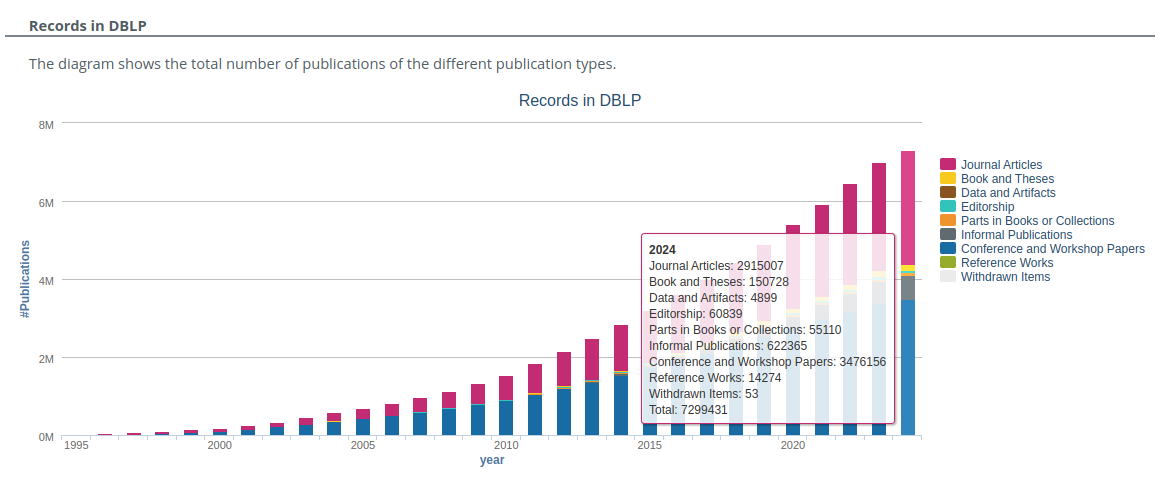
\includegraphics[width=16cm, keepaspectratio]{img/dblp_total_publications_per_year.png}
    \caption{Avance de publicaciones por año.}
    \label{figura:progresion_base_dblp}
 \end{figure}


\section{Historia de dblp.org}
\label{sec:seccion}

El proyecto comenzó de manera modesta, pero experimentó un gran crecimiento debido a una gran demanda de una base de datos accesible y que aportara fiabilidad por parte de la comunidad científica. En un comienzo solo se incluyeron revistas y conferencias clave, expandiendo su alcance rápidamente.

\subsection{Expansión}
Una vez la base de datos comenzó a adquirir adeptos, se trasladó a una plataforma en línea, esto ayudó a incluir un gran numero de nuevas publicaciones, permitió tener un acceso mas amplio y una mayor visibilidad. También se caracterizó en sus comienzos por aplicar características de búsquedas avanzadas.

Es importante tener en cuenta la asociación con otras bases de datos bibliográficas para obtener mas alcance y precisión. Colabora por ejemplo con el IEEE Xplore\footnote{\url{https://ieeexplore.ieee.org/Xplore/home.jsp}} y el ACM Digital Library \footnote{\url{https://dl.acm.org/}}, permitiendo ofrecer referencias cruzadas y enlaces directos a las versiones completas de los artículos cuando estos están disponibles.

\subsection{Importancia}
Dblp ha adquirido la reputación de ser una fuente confiable de información bibliográfica en el ámbito que estamos tratando, ya que mantiene un enfoque en la calidad y precisión en los datos que se muestran. 
Hay que destacar la facilidad de uso como uno de sus aspectos que mas lo caracterizan, posee una interfaz que permite realizar búsquedas precisas, de manera agil y de forma intuitiva, porque puede utilizarse en su búsqueda palabras clave, autores, títulos, conferencias, autor... 

Poseé un gran amplio catálogo de especialidades\footnote{\url{https://dblp.org/faq/1474671.html}}, esto ayuda a los autores de diferentes áreas puedan encontrar publicaciones destacadas y así mantenerse al día con el avance en su propio campo.

Gracias a dblp los autores han conseguido una gran visibilidad debido a tener indexadas las publicaciones, debido a que es muy utilizado por académicos, revisores de revistas y conferencias, comites evaluadores con el fin de evaluar el trabajo de los investigadores. Figurar notablemente en dblp influye de manera positiva en la reputación, reconocimiento abriendo oportunidades para recibir invitaciones a conferencias, oportunidades de colaboración y de revisión de trabajos.

\begin{figure}[h]
    \centering
    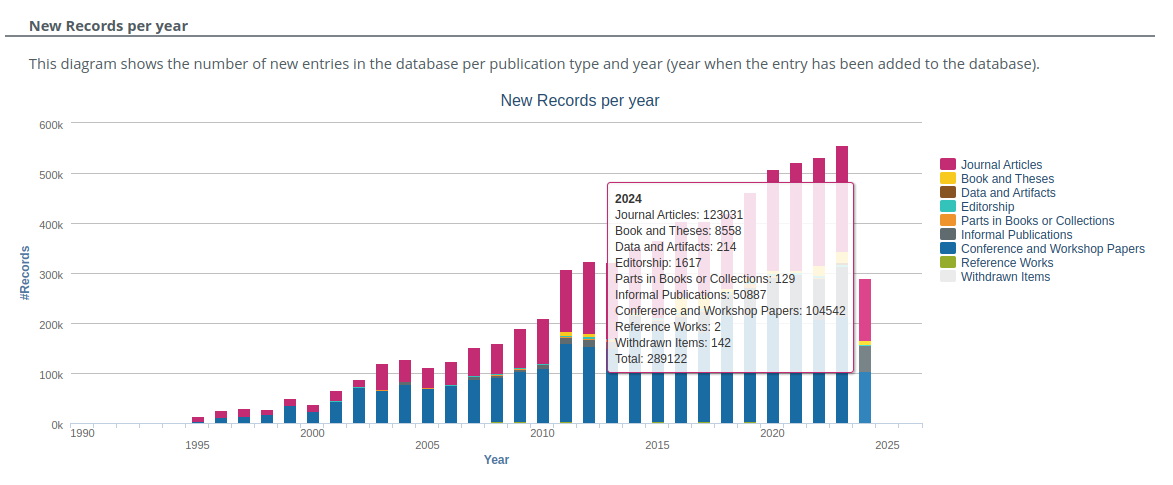
\includegraphics[width=16cm, keepaspectratio]{img/dblp_new_records_per_year.png}
    \caption{Nuevas publicaciones por año.}
    \label{figura:progresion_base_dblp}
 \end{figure}

También dblp proporciona múltiples métricas e indicadores como número de publicaciones, citas recibidas que son consideradas en, por ejemplo, procesos de contratación o financiación de investigaciones, es por ello que es importante tener visibilidad en esta base de datos.

Algo importante de la cual se hace eco este trabajo es la importante red de colaboradores que aparecen, pudiéndose mostrar las conexiones entre autores a través de cooperar en publicaciones.

Cabe destacar el impacto en la educación, ya que es utilizado por educadores y estudiantes para mantenerse actualizados en los últimos avances en su sector.


\section{Estructura de la memoria}
\label{sec:estructura}

Este trabajo se estructura de la siguiente manera:
\begin{enumerate}
    \item \textbf{Introducción}: En este capitulo se pone en contexto la magnitud de dblp y expone el contexto del trabajo.
    \item\textbf{Objetivos}: En este apartado se definen los objetivos generales y los específicos del trabajo, de igual manera se expone la planificación temporal llevada a cabo.
    \item\textbf{Estado del arte.}: En este bloque se detallan las tecnologías utilizadas en el proyecto y se concreta su utilización durante el proceso del trabajo.
    \item\textbf{Diseño e implementación}: En este capítulo se desarrolla el proceso llevado en la implementación de la solución y se detallan los funcionamientos de los códigos que se han desarrollado.
    \item\textbf{Experimentos y validación}: En este apartado se explican las pruebas realizadas y se detalla el funcionamiento de la herramienta de test.
    \item\textbf{Resultados}: En este capítulo se exponen los resultados obtenidos y se realiza la comparación respecto a los valores ofrecidos en los tests.
    \item\textbf{Conclusiones}: En este capítulo se reflexiona sobre los resultados obtenidos y las líneas futuras de trabajo.
    \item\textbf{Apéndice}: En este apartado se van a exponer las capturas de los resultados del capítulo de resultados.
\end{enumerate}


%%%%%%%%%%%%%%%%%%%%%%%%%%%%%%%%%%%%%%%%%%%%%%%%%%%%%%%%%%%%%%%%%%%%%%%%%%%%%%%%
%%%%%%%%%%%%%%%%%%%%%%%%%%%%%%%%%%%%%%%%%%%%%%%%%%%%%%%%%%%%%%%%%%%%%%%%%%%%%%%%
% OBJETIVOS %
%%%%%%%%%%%%%%%%%%%%%%%%%%%%%%%%%%%%%%%%%%%%%%%%%%%%%%%%%%%%%%%%%%%%%%%%%%%%%%%%

\cleardoublepage % empezamos en página impar
\chapter{Objetivos} % título del capítulo (se muestra)
\label{chap:objetivos} % identificador del capítulo (no se muestra, es para poder referenciarlo)

\section{Objetivo general} % título de sección (se muestra)
\label{sec:objetivo-general} % identificador de sección (no se muestra, es para poder referenciarla)


Mi trabajo fin de grado consiste en crear una herramienta de análisis de autores que comparten congresos y revistas utilizando DBLP.
Se pretende entender graficamente I)la cantidad de colaboraciones, y II) las dinámicas de publicacion de los autores por congreso, todo dentro
del marco de la comunidad científica.



\section{Objetivos específicos}
\label{sec:objetivos-especificos}

Este proyecto tiene como objetivo crear una herramienta de análisis de autores coincidentes utilizando DBLP, sin embargo, 
este concepto es lo suficientemente amplio como para abordarlo de manera general.Por lo tanto, los objetivos específicos detallan
de la siguiente manera:

1. Decidir las metodología, que tecnologías y proceso tendrá el ecosistema.

2. Desarrollo de la herramienta de visualización de datos:
Para ello se debe implementar:

- La herramienta extracción de datos, procesamiento y ordenación de los mismos.

- Una interfaz gráfica de usuario (WEB) que facilite la interacción y visualización de los datos.

3. Comparación de la interfaz gráfica con la herramienta de conteo de autores por congreso.







\section{Planificación temporal}
\label{sec:planificacion-temporal}

En este apartado se va a describir el tiempo invertido en este proyecto, como se puede ver en la figura ~\ref{fig:cronograma} se ha empeñado 24 semanas para la definición del tema, análisis del problema, estudio exhaustivo de las tecnologías, implementación del software y la memoria.

\begin{figure}[h]
  \centering
  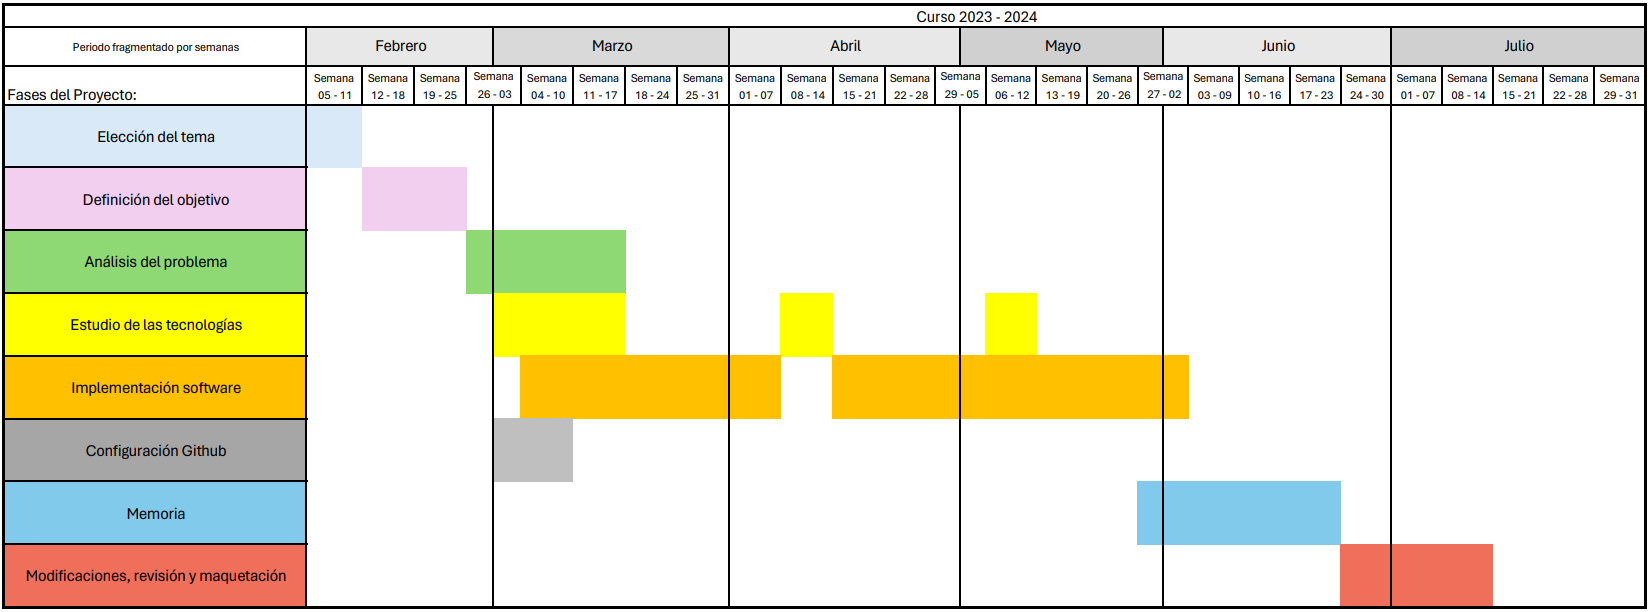
\includegraphics[width=16cm, keepaspectratio]{img/cronograma.png}
  \caption{Cronograma de la creación del proyecto}
  \label{fig:cronograma}
\end{figure}

Durante el comienzo del proyecto en las primeras 5 semanas se hizo un despliegue de 15 horas semanales desglosadas en una hora diaria en el periodo de lunes a viernes y 5 horas diarias durante el fin de semana.

Una vez que se comenzó con la implementación del software, el tiempo empeñado aumentó debido a la complejidad del problema. Se empeñó un total de 20 horas semanales repartidas en una hora diaria entre semana y 7 - 8 horas el fin de semana.

Para la escritura de la memoria, se dispuso de 15 - 20 horas semanales de media.

%%%%%%%%%%%%%%%%%%%%%%%%%%%%%%%%%%%%%%%%%%%%%%%%%%%%%%%%%%%%%%%%%%%%%%%%%%%%%%%%
%%%%%%%%%%%%%%%%%%%%%%%%%%%%%%%%%%%%%%%%%%%%%%%%%%%%%%%%%%%%%%%%%%%%%%%%%%%%%%%%
% ESTADO DEL ARTE %
%%%%%%%%%%%%%%%%%%%%%%%%%%%%%%%%%%%%%%%%%%%%%%%%%%%%%%%%%%%%%%%%%%%%%%%%%%%%%%%%

\cleardoublepage
\chapter{Estado del arte}
\label{chap:estado}

        En este capítulo se van a introducir las tecnologías utilizadas en este trabajo.

\section{Python} 
\label{sec:seccion1}

Python ha adquirido una relevancia como lenguaje de programación mas utilizado en la comunidad académica y científica debido a que se trata de un lenguaje de alto nivel, cuya característica principal es sencillez. La versatilidad y la gran colección de bibliotecas especializadas componen el resto de características mas importantes.

Dentro del contexto de este trabajo, la creación de una herramienta de análisis donde se observa como los autores coinciden en los congresos es muy destacado debido a:

\begin{enumerate}
    \item Extracción y la posterior manipulación de datos: Bibliotecas como sqlite3, lmxl o json nos ayuda a convertir los datos en una base de datos manejable.
    
    \item Web Scraping y APIs: En este apartado destacan las librerías como BeautifulSoup (utilizadas en el comienzo del trabajo) y Request utilizadas para obtención de los datos dentro de la web, incluyendo la recolección de la información de los datos bibliográficos como en este caso DBLP.

    \item Visualización de datos: Bibliotecas como plotly o matplotlib se utilizan para la creación de gráficos detallados de los datos de las publicaciones y colaboraciones entre autores. En este caso se desestimó la idea, ya que como se verá a continuación se desarrolló una herramienta web.
\end{enumerate}

Ventajas de utilizar Python en este proyecto:

\begin{itemize}
    \item Amplia comunidad y soporte: facilidad de acceso a recursos y tutorialesy una amplia comunidad de usuarios y desarrolladores activa.

    \item Eficiencia y simplicidad de uso: Con una sintaxis clara y precisa puedes desarrollar una solución eficiente y rápida.
\end{itemize}

\subsection{SQlite3}

SQLite3 es una librería en Python que proporciona las herramientas para interactuar con la base de datos de SQlite. Dicha base de datos es una bibliteca de C que implementa un motor de bases de datos SQL autónomo, fiable, sin configuración y con todas las funciones de SQL.

La integración con SQL se produce directamente desde python pudiendo utilizar los comandos: 'SELECT', 'INSERT', 'UPDATE', 'DELETE', como otros operadores de las bases de datos.

No precisa de configuración en un servidor independiente, las bases de datos se almacenan en un archivo del sistema de archivos, facilitando el transporte y su uso. Es importante destacar que cada archivo de base de datos es completamente autónomo y contiene los datos y la lógica necesaria para su funcionamiento.

\subsection{Lxlm}

Se trata de una librería de python que tiene como funciones el procesamiento y manipulación de archivos HTML y XML, es una herramienta con mucho potencial que está construida sobre bibliotecas C, concretamente 'libxslt' y 'libxml2'.

Tiene como características principales la facilidad de uso, compatibilidad con HTML5, manipulación de árboles de datos y destacan el rendimiento y velocidad.

En nuestro trabajo se utiliza para realizar el parseo de información hacia la base de datos en formato SQL.

\subsection{Os}

Biblioteca que proporciona una interfaz para interactuar con el sistema operativo base, permitiendo ejecutar comandos propios del sistema operativo de forma portatil. En nuestra herramiente se utiliza para levantar un error del sistema.

\subsection{Argparse}

Se trata de una librería estandar que proporciona las herramientas para definir los argumentos que precisa una interfaz de línea, como deben procesarse y generan la ayuda para los usuarios. Fue incorporado a Python 2.7 como remplazo de optparse

\subsection{Time}

Biblioteca que suministra las funciones para trabajar con el tiempo, pudiéndose implementar funciones como medir el tiempo de ejecución del programa, gestionar marcas de tiempo o incluir retrasos en el código.

En nuestro trabajo se utiliza para medir la cantidad de tiempo que tarda en realizar el parseo del XML de DBLP.

\subsection{Json}

Módulo que proporciona las herramientas necesarias para la manipulación de archivos JSON. En nuestro proyecto se utiliza para crear el JSON que será leido mediante la API.

\subsection{BeautifulSoup}
Librería de Python diseñada para extraer datos de archivos HTML y XML de forma sencilla. Se utiliza para técnicas de scraping.
Tiene como características principales:
Capacidad de manejar documento que no tienen un formato bien definido: Puede analizar archivos HTML que no están estrictamente formados y un así tener la capacidad de extraer los datos de una manera correcta.

Navegación por el arbol de elementos: Permite mediante una API el manejo, selección y modificación de árboles de datos de manera sencilla.

Flexibilidad: Permite elegir entre varios parsers, esto aporta flexibilidad en cuanto a compatibilidad y rendimiento.

Facilidad de implementar: Es facil de usar y aprender, es por ello que se utilizó en un comienzo del proyecto.

Posee una comunidad activa y con buen soporte.

Buena integración con otras herramientas como por ejemplo request o pandas.

\subsection{Request}
Es una biblioteca que te ayuda a realizar peticiones HTTP/1.1. Es utilizada para interactuar con APIs y servicios web, realizando peticiones GET, POST, PUT, DELETE y obteniendo la respuesta de manera efectiva. Cabe destacar varias de las características:

\begin{itemize}
    \item Simplicidad.
    \item Manejo automático de Cookies.
    \item Soporte para HTTPS.
\end{itemize}


\section{JSON} 
\label{sec:seccion1}

JavaScript Object Notation se caracteriza por su simplicidad, legibilidad y compatibilidad con multiples lenguajes de programación, incluyendo como en nuestro caso Python.
Este formato tiene como función almacenar información estructurada que se utiliza para la transferencia de datos entre un servicio web y aplicaciones, principalmente.

Originariamente, JSON se utilizaba con la notación basada en objetos de JavaScript, el formato se compone de dos campos diferenciados key y value.
Las Keys contienen una cadena de caracteres entrecomillada y los Values o valores contienen un tipo de dato válido JSON, del mismo modo entrecomillado. Dicho campo puede estar formado por un array, un string, un objeto, un diccionario, un boolean, un número o un tipo nulo.

En este punto se presenta un ejemplo de la estructura tipo de un formato JSON:

\begin{lstlisting}
{
    "Key": {
        "Dict": {
            "option1": "ok",
            "List": [
                "thing1",
                "thing2",
                "thing3"
            ]
        },
        "Dict2": {
            "opcode": "custom",
            "List2": [
                "customA",
                "customB"
            ]
        }
    }
}
\end{lstlisting}

En el contexto del trabajo, que es la de crear una herramienta de análisis, desempeña un papel fundamental en los siguientes aspectos:

Almacenamiento de datos: Permite almacenar información complicada bien organizada, debido a su estructura flexible y jerárquica. En este trabajo cada autor o publicación se puede almacenar o representar como un objeto JSON con atributos como nombre, año, titulo... Facilitando el manejo y haciéndolo mas accesible.

Intercambio de datos: Como se mencionó anteriormente, es utilizado primordialmente para el intercambio entra servicios web y aplicaciones. La funcionalidad de este trabajo es la de ser extraídos mediante una API, simplificando el análisis y el procesamiento.

Sencillez a la hora de manipular los datos: Se convierte en una tarea mas sencilla debido a la combinación con bibliotecas de Python, que facilitan la escritura, lectura y transformación de la información. 

En conclusión, se trata de un formato muy versatil debido a su compatibilidad multilenguaje, pose flexibilidad y extensibilidad, ya que se puede incorporar nueva información conforme sea necesario y se trata de un formato sencillo y claro a la hora de su visualización.


\section{HTML}

Es el lenguaje utilizado para estructurar y crear páginas web y su contenido. HyperText Markup Languaje fue creado en 1991 y ha ido evolucionando conforme a las necesidades de los usuarios y desarrolladores web.

Desde su comienzo han sido varias las versiones que se han desplegado, destacando HTML 2.0, dicha versión estandarizó muchas funcionalidades y etiquetas que eran soportadas por los navegadores de la época. La versión HTML 4.0 en la cual se introdujo las hojas de estilo CSS. Y la más conocida y actual HTML5, que data del 2014, dicha versión se caracteriza por la inclusión de nuevas etiquetas que dan soporte nativo a las fuentes multimedia, mejora de formularios y soporte para APIs avanzadas.

El impacto provocado por esta versión se caracteriza por la transformación de como se interactua con el contenido en linea. A continuación se detalla las tendencias actuales y futuras que dan forma a la web:

\textbf{Mejoras en posicionamiento SEO y accesibilidad:} Con la incorporación de nuevas etiquetas y atributos permiten a los desarrolladores crear webs que tengan mejor posicionamiento y visibilidad en motores de busqueda y tambien ayuda a ser mas accesibles para personas con discapacidades.

\textbf{Interactividad con WebXR:} Esta tendencia ayuda a abrir nuevas soluciones para interactuar y sumergirte en la web, con la API WebXR ayuda a crear experiencias de realidad virtual (VR) y de realidad aumentada (AR).

\textbf{Aplicaciones web progresivas (PWA):} Esta opción es muy popular entre los desarrolladores que buscan crear aplicaciones que puedan ser utilizadas desde cualquier dispositivo que disponga de un navegador.

\textbf{WebAssembly:} es una tecnología que permite ejecutar codigo de bajo nivel como si se ejecutar de manera nativa. Se utiliza por ejemplo para ejecutar juegos, aplicaciones de calculo o software de edición como si de una aplicación nativa se tratara.

\section{CSS3}
Cascading Style Sheets u hojas de estilo en cascada define como se debe visualizar los elementos de HTML. Está diseñado para discretizar el contenido del documento y la forma de visualizarse dichos datos, se pueden aplicar características tales como los colores, fuentes y capas o layouts.

Se le denomina estilos de cascada ya que se aplican las características de forma jerárquica (de arriba a abajo) siguiendo un patrón de herencia.

\section{NODEJS}

Es un entorno de ejecución de JavaScript implementado bajo el motor de Google Chrome V8, revolucionando el desarrollo de aplicación en la parte del servidor, permitiendo a los desarrolladores utilizar JavaScript tanto en Back-end como en Front-end. Es extremadamente escalable y eficiente para aplicaciones web y servidores puesto que su arquitectura está orientada a eventos y por su modelo de entrada/salida no bloqueante.

Las características principales son:

\begin{itemize}
    \item Arquitectura Orientada a Eventos: Utiliza un bucle de eventos para controlar multiple conexiones simultaneas sin necesidad de establecer nuevos hilos de procesamiento.
    \item Modelo de entrada/salida no bloqueante: Realiza operaciones entrada/salida de manera asíncrona, permitiendo no bloquear el hilo principal.
    \item NPM: Es una colección de modulos y bibliotecas que los desarrolladores pueden utilizar.
    \item Compatibilidad con JSON: Implementa la creación y consumo de APIs RESTful.
    \item Servidor HTTP integrado: Facilidad de crear un servidor web sin necesidad de otros entornos mas complejos como Nginx o Apache.
\end{itemize}

\section{dblp.org}
Las siglas corresponden con "Digital Bibliography \& Library Project", se trata de una base de datos en linea que proporciona información sobre las principales publicaciones dentro del mundo de la informatica de forma bibliográfica. Se incluyen conferencias, artículos de revistas y publicaciones académicas. 

\begin{figure}[h]
  \centering
  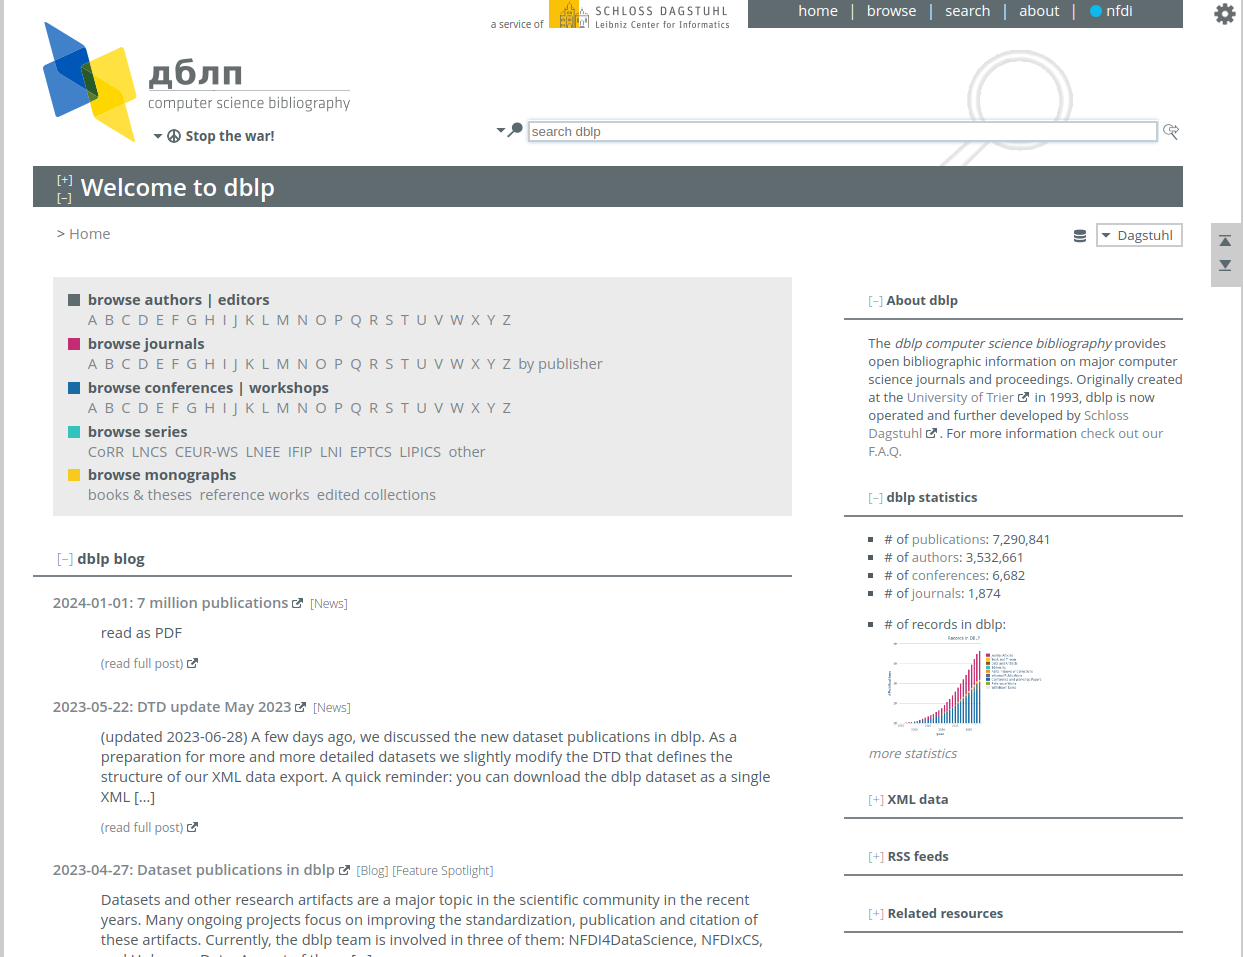
\includegraphics[width=16cm, keepaspectratio]{img/dblp_frontpage.png}
  \caption{Página principal de la web dblp.org}
  \label{fig:web}
\end{figure}
%¿????????????????????????????????????????????????????????????????%
% REVISAR LA CITA%
%¿????????????????????????????????????????????????????????????????%
Según datos de la web: \" En enero de 2024, dblp indexa más de 7 millones de publicaciones, publicadas por más de 3,4 millones de autores. Con este fin, dblp indexa alrededor de 55.000 volúmenes de revistas, más de 55.000 actas de congresos y talleres y más de 140.000 monografías."

\section{Inloop.github.io/sqlite-viewer/}

Se trata de un visor de bases de datos online, es una herramienta de Inloop, la cual acepta archivos con extensión .db y permite realizar las mismas acciones que se llevan a cabo en cualquier gestor de bases de datos de SQLite. Se puede ver un ejemplo de visualización de los datos en la figura ~\ref{fig:ej_bd}.

%%%%%%%%%%%%%%%%%%%%%%%%%%%%%%%%%%%%%%%%%%%%%%%%%%%%%%%%%%%%%%%%%%%%%%%%%%%%%%%%
%%%%%%%%%%%%%%%%%%%%%%%%%%%%%%%%%%%%%%%%%%%%%%%%%%%%%%%%%%%%%%%%%%%%%%%%%%%%%%%%
% DISEÑO E IMPLEMENTACIÓN %
%%%%%%%%%%%%%%%%%%%%%%%%%%%%%%%%%%%%%%%%%%%%%%%%%%%%%%%%%%%%%%%%%%%%%%%%%%%%%%%%

\cleardoublepage
\chapter{Diseño e implementación}
\label{sec:diseno}

En este capítulo se va a describir la estructura del software desarrollado, como se han utilizado las herramientas descritas en el apartado anterior.

\section{Arquitectura general} 
\label{sec:arquitectura}

Para la consecución de este proyecto debemos tener en cuenta la transformación de formatos que va aplicando los datos, para conocer que software o código se ha ido implementando.


Dicha figura~\ref{fig:arquitectura} refleja como se van convirtiendo y segmentando los datos para poder visualizados en un navegador web.

\begin{figure}[h]
  \centering
  
\includegraphics[width=16cm, keepaspectratio]{img/esquemadatos_com.png}
  \caption{Estructura de transformación de los datos}
  \label{fig:arquitectura}
\end{figure}

% Mas tarde haremos incapié en esta figura para poder ponernos en contexto dentro del proyecto.

\section{Desglose general de la solución} 

El proceso que se ha de seguir para obtener los datos graficados son los siguientes:

Descarga de los archivos de la web de dblp.org, se puede realizar haciendo click sobre los siguientes enlaces:
\begin{verbatim}    
https://dblp.org/xml/dblp.dtd
https://dblp.org/xml/dblp.xml.gz
\end{verbatim}
O por el contrario si te encuentras en un entorno Linux puedes descargarlo mediante el comando:
\begin{verbatim}
wget https://dblp.org/xml/dblp.dtd
wget https://dblp.org/xml/dblp.xml.gz
\end{verbatim}
Esto nos descarga un archivo .gz (archivo comprimido) y un archivo en formato .dtd, para el manejo de los datos es necesario realizar una descompresión del archivo "dblp.xml.gz", para ello se debe utilizar el comando:
\begin{verbatim}
gzip -d dblp.xml.gz
\end{verbatim}
En este punto nos encontramos en la segunda posición de la figura ~\ref{fig:bs_extract}, es momento de convertir o parsear los datos para hacerlos manejables mediante:
\begin{verbatim}
python3 main_dblp_parser.py --dblp dblp.xml --output DBLP.db
\end{verbatim}
Nos situamos en la tercera posición de la figura ~\ref{fig:bs_extract}, es fundamental trabajar únicamente con los datos que necesitamos, es por ello que sintetizamos los registros de la base de datos en formato .db en los datos únicos con los que vamos a realizar las operaciones. Para ello debemos de utilizar la funcion:

\begin{verbatim}
python3 extraccion_datos_concretos.py
\end{verbatim}
Con dicha función obtenemos un JSON que divide los congresos por diccionarios, consiguiendo la información precisa con la que vamos a alimentar nuestra web. En este punto ejecutamos un servidor API para surtir con los datos a la web, mediante el comando:
\begin{verbatim}
json-server --watch out.json --port 4400
\end{verbatim}
Obteniendo una captura como en la figura ~\ref{fig:json_server}, es en este momento cuando se puede visualizar el contenido del archivo index.html. Teniendo un ejemplo de los resultados en la figura ~\ref{fig:res_web}, presentando los autores por orden de aparición en cada congreso.

Tras esto, se van a detallar las configuraciones para poder realizar estos pasos.

\begin{figure}[h]
  \centering
  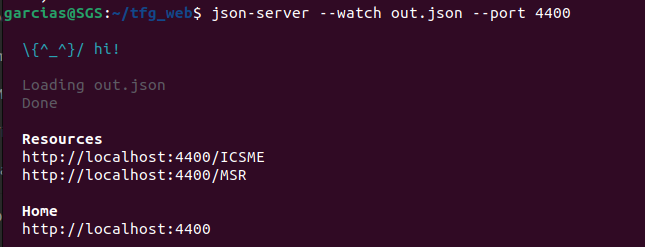
\includegraphics[width=15cm, keepaspectratio]{img/terminal_json_server.png}
  \caption{Salida terminal json-server}
  \label{fig:json_server}
\end{figure}

\subsection{Extracción de datos directamente desde la web de DBLP.org}

En este primer apartado se va a desarrollar como comenzó en este trábajo con el tratamiento de los datos, la primera aproximación a buscar una solución al problema propuesto fue la de obtener los datos directamente de la web, es por ello que se implementa el primer código: \textit{BS\_extract.py}

\begin{figure}[h]
  \centering
  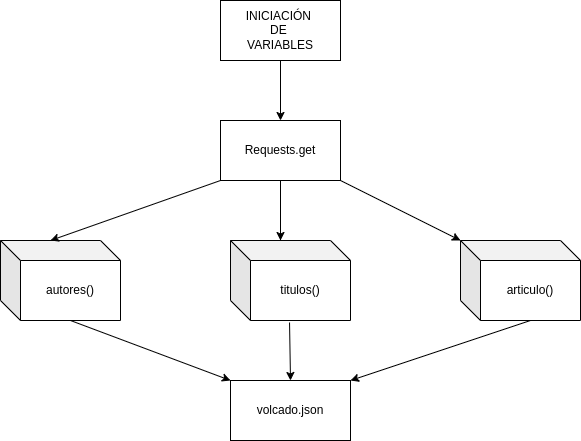
\includegraphics[width=12cm, keepaspectratio]{img/BS_extract_graph.png}
  \caption{Estructura del código BS\_extract.py}
  \label{fig:bs_extract}
\end{figure}

Como se puede observar en la figura ~\ref{fig:bs_extract}, el código está diseñado para extraer información del portal dblp utilizando la petición requests, la cual realiza una petición HTTP, mediante las herramientas de la librería BeautifulSoup maneja los datos obtenidos por medio de  las etiquetas html. Es por ello que se desarrollan 3 funciones:

\begin{itemize}
    \item \textbf{Autores():}
    en dicha función se comprueba que la respuesta ha sido correcta, devolviendo un \textit{estatus\_code} igual a 200. A continuación, el código hace una búsqueda por "name", esto devuelve un árbol con los datos extraídos.
    Se recorre dicha variable para evitar los autores que no dispongan de "title", mas tarde se ordena el diccionario para volcarlo al archivo volcado.json.
    \item \textbf{Titulos():}
    como en el caso anterior, lo primero que comprueba es si se ha tenido éxito en la petición HTTP, La particularidad que posee esta función es que extráe todos los títulos de los artículos que aparecen en la URL que le pasamos como parámetro.
    \item \textbf{Articulos():}
    tiene como objetivo extraer los artículos junto con los autores. La primera busqueda que se realiza es apuntando a la etiqueta \textit{cite}. Afinando una vez que tenemos los datos de dicha etiqueta, los títulos por medio de la etiqueta \textit{tittle} y los autores por medio de la etiqueta \textit{name}. En la figura ~\ref{fig:bs_ej} se observa un ejemplo del resultado dentro del volcado de la información.
\end{itemize}

\begin{figure}[h]
  \centering
  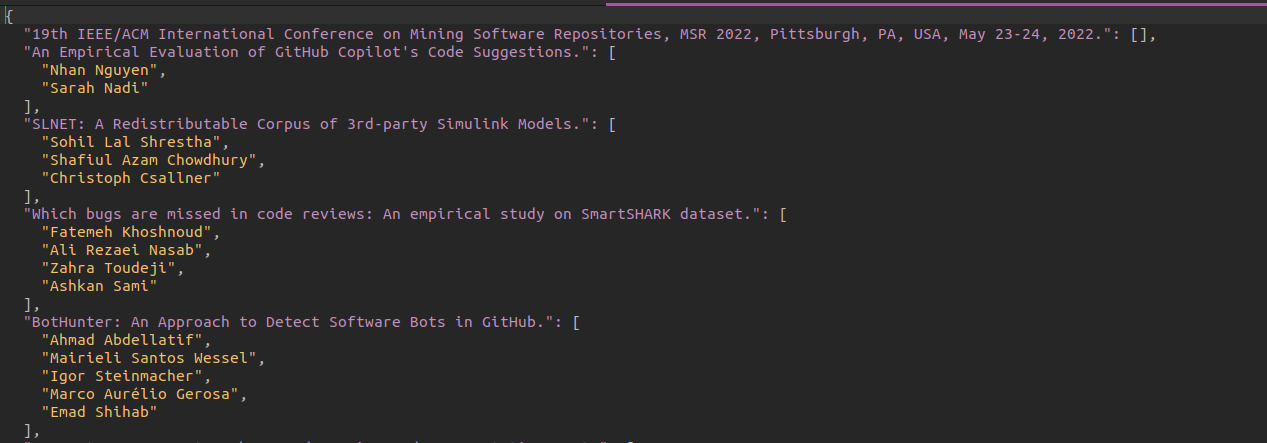
\includegraphics[width=16cm, keepaspectratio]{img/ej_salida_BS.png}
  \caption{Ejemplo de salida de Autores(), dentro del archivo volcado.json}
  \label{fig:bs_ej}
\end{figure}

Con esta implementación se observó que no se disponía de todos los datos que se necesitan para cada conferencia. Es necesario repetir el proceso para cada URL que contenga información de los congresos que se van a comparar.

Esta primera configuración nos dió visibilidad de la magnitud real del problema a abordar. Se tomo conciencia de la necesidad de ir directamente a la fuente de los datos. Aunque esta primera configuración se dejó aparcada, sirvió como un valioso aprendizaje para comprender y conocer BeautifulSoup, pronto se notó que no proporcionaba resultados fiables.

Es por ello que se procedió a implementar una configuración complementaria que acabaría siendo el resultado final de este trabajo.

\subsection{Tratamiento de datos XML y guardado en base de datos}

Una vez identificada la magnitud del problema, necesitamos el tratamiento de los datos en un soporte accesible como las bases datos. Con esta transformación se buscó poder aplicar las órdenes básicas de SQL y hacer manejable la ingente cantidad de datos.

Para ello se lleva a cabo la implementación de \textit{main\_dblp\_parser.py}:

El codigo está diseñado para procesar un archivo XML y almacenar la información en una base de datos SQLite, aprovechando la librería lmxl para el análisis y manipulación del XML y SQLite3 para la gestión de bases de datos.

Para ello se debe de ejecutar el código por términal:

\begin{verbatim}
python3 main_dblp_parser.py --dblp dblp.xml --output DBLP.db 
\end{verbatim}

Ambos parámetros exigidos ya que recogen los datos necesarios para el correcto funcionamiento.

Desglosando los parámetros:

--dblp (archivo) nos exige que introduzcamos la ruta del archivo XML que vamos a utilizar y parsear para convertirlo en base de datos.

--output (archivo) en este caso le debemos de introducir el nombre del archivo con extensión que obtendrémos al final la ejecución de dicho software. 

Una vez pasamos los parámetros se va inicializar un contador (star\_time), ayudando a conocer el tiempo concreto de ejecución, dicho tiempo varía conforme a los recursos de la máquina en la cual se ejecuta, en el apartado de resultados se va a llevar a cabo una comparativa de tiempo, dependiendo del ordenador en el que se ejecuta. 
Una vez se ha inicializado el contador, obtenemos la función central de la solución del parseo del XML. 

\begin{figure}[h]
  \centering
  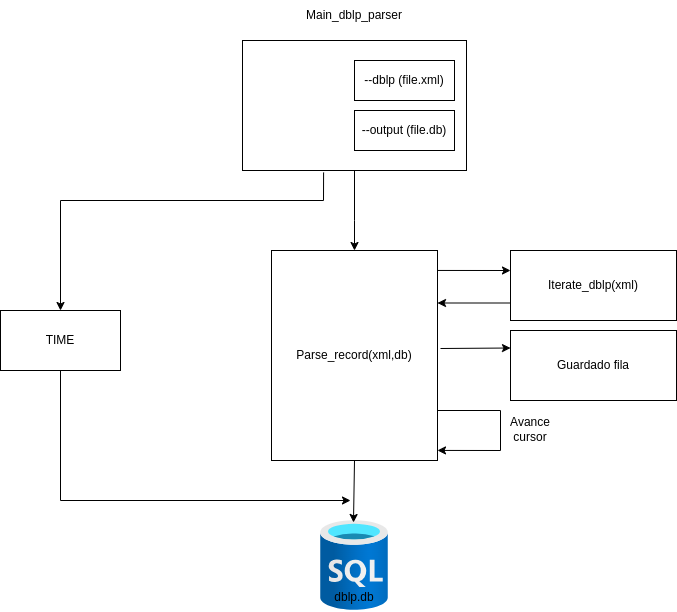
\includegraphics[width=15cm, keepaspectratio]{img/main_dblp_parser_par.png}
  \caption{Esquema general parsers}
  \label{fig:dblp_parser}
\end{figure}

\subsubsection{Parse\_record():}

En ese momento se ejecuta el parametro \textit{parse\_record(dblp.xml, output.db)}, es importante destacar la inicialización de la base de datos si no existiera bajo el comando: 

\begin{verbatim}
    c.execute("""CREATE TABLE IF NOT EXISTS records
            (id INTEGER PRIMARY KEY AUTOINCREMENT, 
            genre TEXT, title TEXT,
            author TEXT, year TEXT, 
            booktitle TEXT, ee TEXT, 
            crossref TEXT,url TEXT)""")
\end{verbatim}

En el código anterior se puede apreciar los campos que se van a rellenar con los datos extraidos del XML, se procesan los datos mediante el bucle que hace llamada a la función \textit{iterate\_dblp(dblp)} (explicado mas adelante). 

Una vez se obtienen los datos, se extraen los atributos que se encuentran dentro del record, discretizando los datos, obviando los que se encuentran dentro del listado ignore\_fiel, agregando el texto del atributo a la lista correspondiente en attrs, bajo la orden:

\begin{verbatim}
    attrs[attr.tag].append(attr.text)
\end{verbatim}

Una vez tenemos los datos localizados, se incluyen en la fila de la base datos bajo el comando de SQLite:\textit{ INSERT INTO records (genre, title, author, year, booktitle, ee, crossref, url) VALUES (?,?,?,?,?,?,?,?), (los valores separados por comas).}

En este punto se realiza un volcado de la fila con datos en la base datos, realizando un commit, el siguiente paso es avanzar el cursor para que la siguiente ejecución no sobrescriba los datos y añada a continuación.

Una vez que termina el documento XML, se obtiene la base datos completa, se puede ver un ejemplo en la figura ~\ref{fig:ej_bd}, que muestra varias filas dentro de la tabla 'records'.

\begin{figure}[h]
  \centering
  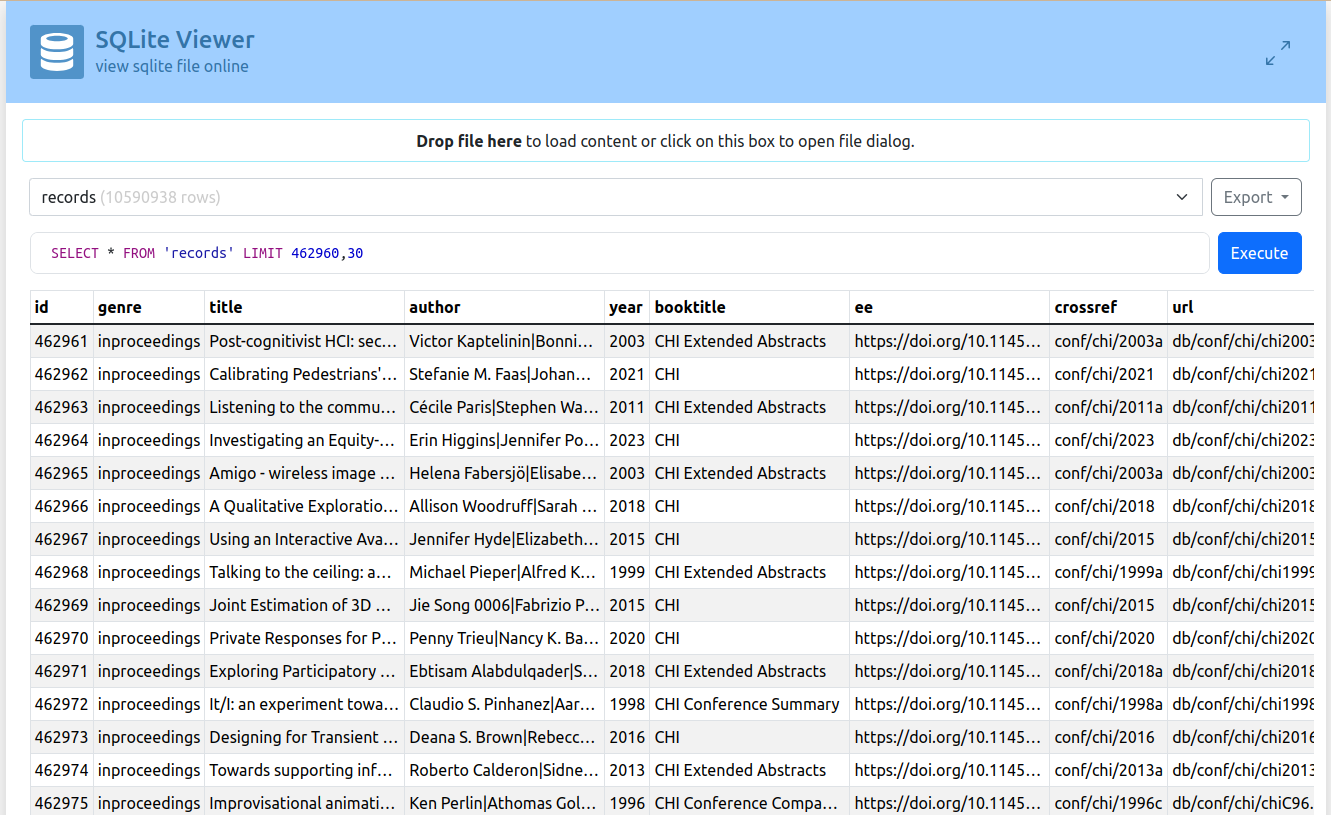
\includegraphics[width=15cm, keepaspectratio]{img/ej_bd.png}
  \caption{Esquema general parsers}
  \label{fig:ej_bd}
\end{figure}

\subsubsection{Iterate\_dblp(dblp)}

Esta función se utiliza para manejar de manera efectiva archivos grandes XML, se realiza por bloques sin necesidad de cargar el documento de una vez, ya que la ocupación en memoria sería alta. Es por ello que se decidió el uso de dicha función en este trabajo.

La función comienza inicializando el iterador etree.iteparse. Concretamente se inicializa aportando la información del archivo que se va a iterar, los eventos que queremos recibir ('start, 'end') y habilitando la validación DTD para asegurar que el documento cumple con el formato.

Lo siguiente que se lleva a cabo es la obtención de la raíz del documento, y se inicializa la variable "star\_tag".

En este punto se va a comenzar a iterar sobre los elementos y eventos, se va a buscar la etiqueta "start" hasta que se encuentre la etiqueta " end", es en este punto cuando tenemos constancia que se trata de un elemento completo, devolviéndolo a la función principal. Inicializa de nuevo la variable "star\_tag" y realiza un limpiado de la raíz del documento para liberar memoria.


\subsection{Extracción de datos concretos a JSON}
Tal y como se aprecia en la figura~\ref{fig:arquitectura}, pasamos al tercer paso del proyecto, en este punto manejamos los datos con consultas a la base de datos bajo el lenguaje SQLite. 

Consta de una función principal que necesita conocer los parámetros: base de datos de entrada, archivo JSON de salida y la fuente de datos a buscar.

La función principal es denominada db\_to\_json(in.db, out.json, datos), consulta una base de datos SQLite para registros que coinciden con valores "booktitle", convierte los datos en un diccionario y guarda los datos en un JSON, haciendo una gestión efectiva de los recursos de la base datos.

El codigo comienza estableciendo la conexión con la base de datos y creando un cursor para ejecutar consultas SQLite. Del mismo modo se inicializa el diccionario 'datos\_json' para almacenar los datos que mas tarde serán volcados sobre el archivo JSON.

Se realiza una consulta a la tabla 'records' para obtener los registros coincidentes 'booktitle' iguales a 'dato':

\begin{verbatim}
cursor.execute("SELECT * FROM 'records' 
    WHERE booktitle = '{dato}'".format(dato=dato))
\end{verbatim}

Dichos datos se obtienen mediante el 'cursor.fetchall()', es en este punto donde manejamos los datos inicializando una lista denominada 'registros', creando un diccionario por cada fila obtenida de la consulta. Es en este punto cuando se cierra la conexión con la base de datos.

Una vez que se ha iterado sobre todos los datos, se vuelca los datos al archivo JSON.

\begin{verbatim}
    with open(filejson, 'w') as archivo_json:
        json.dump(datos_json, archivo_json, indent=4)
\end{verbatim}

\subsection{Visualización de datos}

Para llegar a visualizar los datos como en la figura~\ref{fig:res_web}, se debe de lanzar una API, tal y como se detalla en el apartado 4.2, utilizada debido a su flexibilidad, facilidad de uso, eficiencia en cuanto a la cantidad de datos transferidos mediante respuestas estructuradas y claras.

\subsubsection{Index.html}
Se compone de una etiqueta \textit{head} en la que se encuentran los datos de encriptación y características como fuentes de las letras y la hoja de estilo.

También se compone de una etiqueta general \textit{body}, aquí se encuentra todo el contenido que se va a mostrar por pantalla, la información se encuentra dentro de la etiqueta \textit{main}, la cual está compuesta, por un encabezado formado por el título, un selector de años y 3 secciones que incluyen los gráficos.

Todo ello no muestra ningún dato por si solo, necesita de JavaScript, que obtiene los datos de la API y generan los gráficos.

\subsubsection{App.js}
Script que se encarga de obtener los datos de dos fuentes, cuenta la frecuencia de los autores en dichos datos y muestra la información en forma de gráfico. Chart.js es la librería utilizada para generar los gráficos y hacerlo interactivo. 

A tener en cuenta en este documento es la función principal, en la cual se obtiene los datos desde la API y se pasa como parámetro a las funciones que lo contiene: \textit{printchart()}.

La función \textit{renderAuthorsChart()} se encarga de recoger los datos de ICSME, leer el parámetro author, dividir los autores separados por "\textbar" , inicializando el autor si no se encuentra e incrementando el contador para los autores que si se encuentran.

A continuación se ordena los valores según el número de apariciones de mayor a menor y se le pasa los datos a la función que construye el gráfico, siendo de tipo \textit{'doughnut'}.


La función \textit{renderAuthorsChart2()} recoge los datos de MSR, realiza las mismas operaciones que la función anterior con la peculiaridad que el gráfico es de tipo \textit{'polar'}


La última función de este documento se trata de \textit{renderAuthorsVennChart}, la cual recoge los datos de MSR y ICSME, obtiene las apariciones por autor y congreso, realiza la intersección y muestra un gráfico de tipo \textit{'venn'}.

\begin{figure}[h]
  \centering
  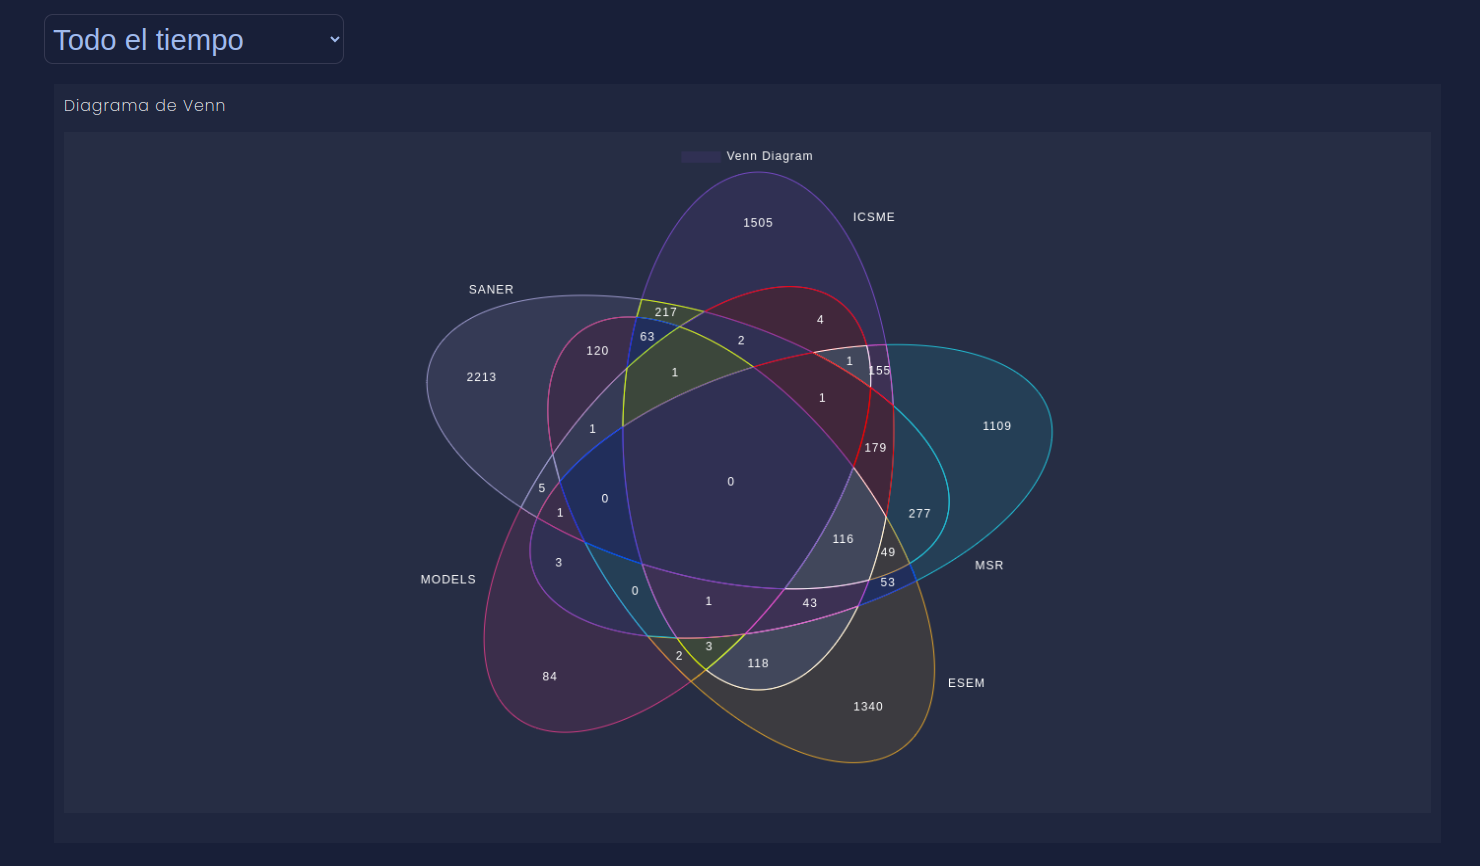
\includegraphics[width=15cm, keepaspectratio]{img/venn_graph_T.png}
  \caption{Diagrama de Venn general}
  \label{fig:venn_graph_t}
\end{figure}

\subsubsection{Helpers.js y Handlers.js}

Estos documentos son utilizados para ayudar a componer el código principal, en primer lugar tenemos \textit{"helpers.js"} el cual alberga funciones necesarias para implementar el código.

\begin{itemize}
    \item FetchAuthorsData: se encarga de realizar las peticiones HTTP a varias URLs las cuales se proporcionan como argumentos y se devuelve una promesa que se resuelve cuando todas las peticiones se han llevado a cabo con éxito.
    \item GetDataColor: se encarga de generar un array de colores y aplicar una opacidad a cada color, si este fuera necesario.
    \item UpdateChartData: es la función que realiza la actualización de los gráficos en tiempo real, permitiendo una visualización dinámica y actualizada de datos. Forma un papel importante cuando se selecciona una opción del select dentro del index.
\end{itemize}
Por otro lado tenemos las funciones de la librería \textit{'Handlers.js}, en la cual se encuentra:

\begin{itemize}
    \item EnableEventHandler: dicha función se encarga de obtener la opción seleccionada en el selector del index (figura ~\ref{fig:selector}), según la opción del desplegable, se selecciona la función \textit{'filterAuthorsByYears'} con distintos parámetros.

    \item FilterAuthorByYears:Realiza un filtrado de los datos por año de comienzo y el número de años previos que debe revisar. Obtiene los autores y busca primero por año, una vez ha encontrado el año realiza el split de los autores como se mencionó anteriormente y posteriormente se cuantifica cuando un autor se encuentra bajo estos parámetros. Devuelve los datos bajo el parámetro \textit{sortedAuthors}
\end{itemize}

\begin{figure}[h]
  \centering
  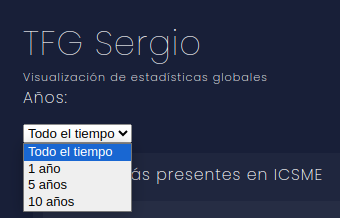
\includegraphics[width=8cm, keepaspectratio]{img/selector.png}
  \caption{Selector de visualización}
  \label{fig:selector}
\end{figure}



%%%%%%%%%%%%%%%%%%%%%%%%%%%%%%%%%%%%%%%%%%%%%%%%%%%%%%%%%%%%%%%%%%%%%%%%%%%%%%%%
%%%%%%%%%%%%%%%%%%%%%%%%%%%%%%%%%%%%%%%%%%%%%%%%%%%%%%%%%%%%%%%%%%%%%%%%%%%%%%%%
% EXPERIMENTOS Y VALIDACIÓN %
%%%%%%%%%%%%%%%%%%%%%%%%%%%%%%%%%%%%%%%%%%%%%%%%%%%%%%%%%%%%%%%%%%%%%%%%%%%%%%%%

\cleardoublepage
\chapter{Experimentos y validación}
\label{chap:experimentos}

En este capítulo vamos a detallar la herramienta que se utiliza para validar los datos que se visualizan en la web del proyecto. Se ha llevado un código en Python que extrae los datos como la herramienta de visualización de datos.

Dicha herramienta tiene por nombre \textit{comparacion\_autores.py} y se va a desarrollar el funcionamiento conforme a la figura~\ref{fig:s_c_p_y}.
\section{\textit{Authors\_year:}}
Esta función tiene como objetivo principal, cosechar los datos conforme a lo necesitado, siguiendo el siguiente formato:
\begin{lstlisting}
{
    "Author1": ["appearances", ["year1","year2",...]],
    "Author2": ["appearances", ["year1","year2",...]],
        ...
    }
\end{lstlisting}

Los datos que se extraen se obtienen por medio del archivo JSON que se pasa como parámetro, una vez obtiene los datos, realiza una comprobación:
\begin{itemize}
    \item Si no se encuentra el autor en el diccionario, se incluye el autor, se inicializa con el valor 1 y se añade el año que ha obtenido.
    \item Por el contrario si el autor se encuentra en el diccionario, aumenta el contador en el primer valor de la lista y añade el valor del año como \textit{append} en la lista dedicada.
\end{itemize}

Termina la ejecución de la función devolviendo el diccionario.

\section{\textit{Authors\_per\_year:}}
Esta función tiene como objetivo extraer el numero de veces que aparece en un año dado, dicho dato se obtiene a través de un parámetro denominado \textit{year}.

Llama a la función anterior para obtener los datos de los autores, habiendo sido filtrado por numero de apariciones y años y realiza una búsqueda en la lista de años. Sumando +1 en caso de que encuentro dicho valor por este usuario.

El resultado se devuelve bajo la orden return.

\section{\textit{Authors\_some\_year:}}

Dicha función extrae los datos en una franja de tiempo, siendo el año de comienzo el parámetro \textit{start\_year} y el valor final de años viene determinado con la cantidad de años a revisar con el parámetro \textit{num\_years} .

Hace una llamada a la función anterior para obtener los años discriminados y realiza el cálculo de los años que aparecen por autor.

Se devuelve el resultado bajo la orden \textit{return resultados}.

\section{\textit{Search\_comparison\_per\_year:}}
Para finalizar y como se puede observar en la figura~\ref{fig:s_c_p_y}, se obtiene la intersección de apariciones de los autores en un intervalo de años, obteniendo su totalidad pasándo como parámetros el año actual y el valor total de años desde 1993, siendo el comienzo de DBLP.

Tal y como se muestra en la figura, hace una llamada a las funciones anteriores tal y como se detallan en los epígrafes previos, realizando una operación intersección y mostrando los valores por terminal.


\begin{figure}[h]
  \centering
  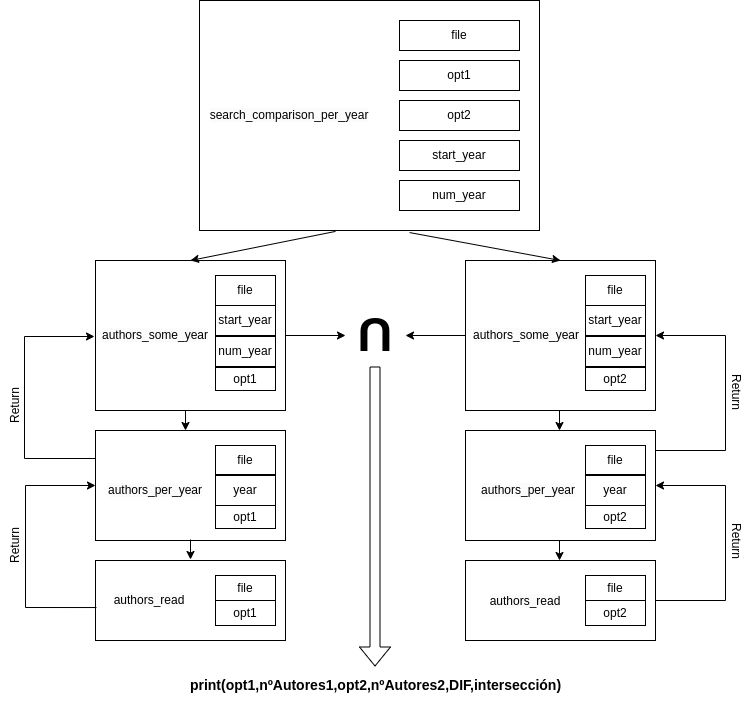
\includegraphics[width=16cm, keepaspectratio]{img/s_c_p_y.png}
  \caption{Esquema general intersección autores}
  \label{fig:s_c_p_y}
\end{figure}
%%%%%%%%%%%%%%%%%%%%%%%%%%%%%%%%%%%%%%%%%%%%%%%%%%%%%%%%%%%%%%%%%%%%%%%%%%%%%%%%
%%%%%%%%%%%%%%%%%%%%%%%%%%%%%%%%%%%%%%%%%%%%%%%%%%%%%%%%%%%%%%%%%%%%%%%%%%%%%%%%
% RESULTADOS %
%%%%%%%%%%%%%%%%%%%%%%%%%%%%%%%%%%%%%%%%%%%%%%%%%%%%%%%%%%%%%%%%%%%%%%%%%%%%%%%%

\cleardoublepage
\chapter{Resultados}
\label{chap:resultados}

En este capítulo se va a describir todos los resultados que se consigue sobre el proceso de creación del proyecto. Vamos a hacer referencia a la figura ~\ref{fig:arquitectura} y vamos a exponer los resultados de cada apartado.
Para comenzar, se va a tener muy en cuenta el tiempo de ejecución del parseo del XML a base de datos, es por ello que según la figura ~\ref{fig:comparativa_pc} podemos ver una gran diferencia en el tiempo de procesamiento. Se muestran en la comparativa los valores que a mi parecer encuentro mas relevantes.

\begin{figure}[h]
    \centering
    \begin{tabular}{cc}
    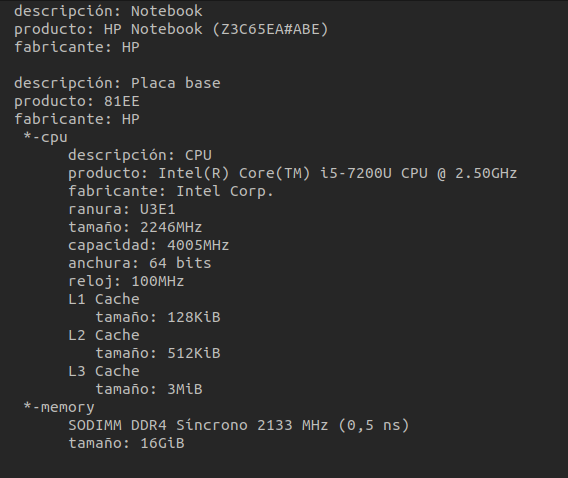
\includegraphics[width=0.46\textwidth]{img/pc_s.png} &  
    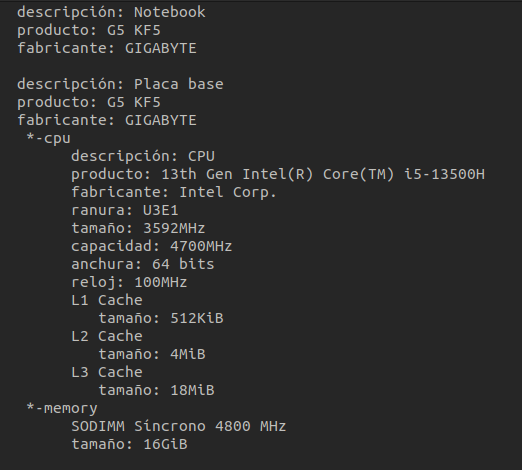
\includegraphics[width=0.44\textwidth]{img/pc_b.png} \\
    (a) &(b)
    \end{tabular}
    \caption{Comparativa de recursos de PC}
    \label{fig:comparativa_pc}
\end{figure}

Como se aprecia en la imagen de la izquierda, se dispone de un Intel i5 de 7º generación(equipo con el que se ha realizado el trabajo) con 16gb de RAM DDR4 con una velocidad de 2333MHZ. Muy diferente al otro equipo que se trata de un procesador i5 de 13º generación(equipo cedido para la prueba) que dispone de una memoria RAM de 16gb a 4800MHZ, es notable la diferencia entre ambos equipos, ya que ambos equipos disponen de Ubuntu 22.04.

\begin{figure}[h]
  \centering
  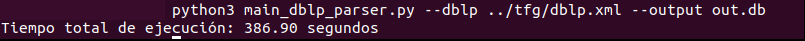
\includegraphics[width=16cm, keepaspectratio]{img/ej_time_i5_7a.png}
  \caption{Tiempo de ejecución i5 7º generación}
  \label{fig:time_s}
\end{figure}
\begin{figure}[h]
  \centering
  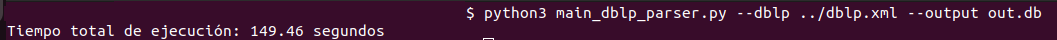
\includegraphics[width=16cm, keepaspectratio]{img/ej_time_i5_13a.png}
  \caption{Tiempo de ejecución i5 7º generación}
  \label{fig:time_b}
\end{figure}

En este punto se puede observar que los componentes del sistema interfieren notablemente en el tiempo de procesamiento, viéndose incrementado el tiempo en un 259\%.



\begin{figure}[h]
    \centering
    \begin{subfigure}{\textwidth}
        \centering
        
\includegraphics[width=0.6\textwidth]{img/tamaño_xml.png} % Reemplaza con tu imagen
        \caption{Tamaño archivo XML}
        \label{fig:xml_tam}
    \end{subfigure}
    \vspace{0.5cm} % Espacio vertical entre las subfiguras
    \begin{subfigure}{\textwidth}
        \centering
        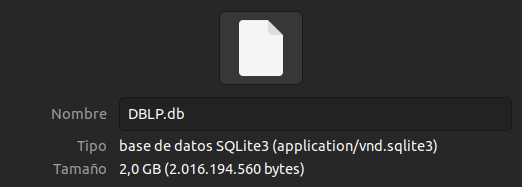
\includegraphics[width=0.6\textwidth]{img/tamaño_db.png} % Reemplaza con tu imagen
        \caption{Tamaño archivo DB}
        \label{fig:db_tam}
    \end{subfigure}
    \caption{Diferencia de tamaños de los datos.}
    \label{fig:tamaños}
\end{figure}


Otro resultado a tener en cuenta es la salida del parseo del XML, se trata de la diferencia de espacio en disco ocupa el origen de los datos (el archivo XML) respecto al guardado en la base de datos extrayendo los datos que se determinaron como relevantes. Se observa de una diferencia de compresión de espacio en disco de 2.1 veces. 


Es importante este dato, ya que el manejo de la información en origen era insostenible para un trabajo de esta magnitud. Además que se pueden realizar peticiones a la base de datos y extraer los datos concretos para que así afinar mas la información.

Se puede ver un ejemplo en la figura ~\ref{fig:ej_sqlite}, como se puede concretar la información con una simple orden en SQLite:

\begin{figure}[h]
  \centering
  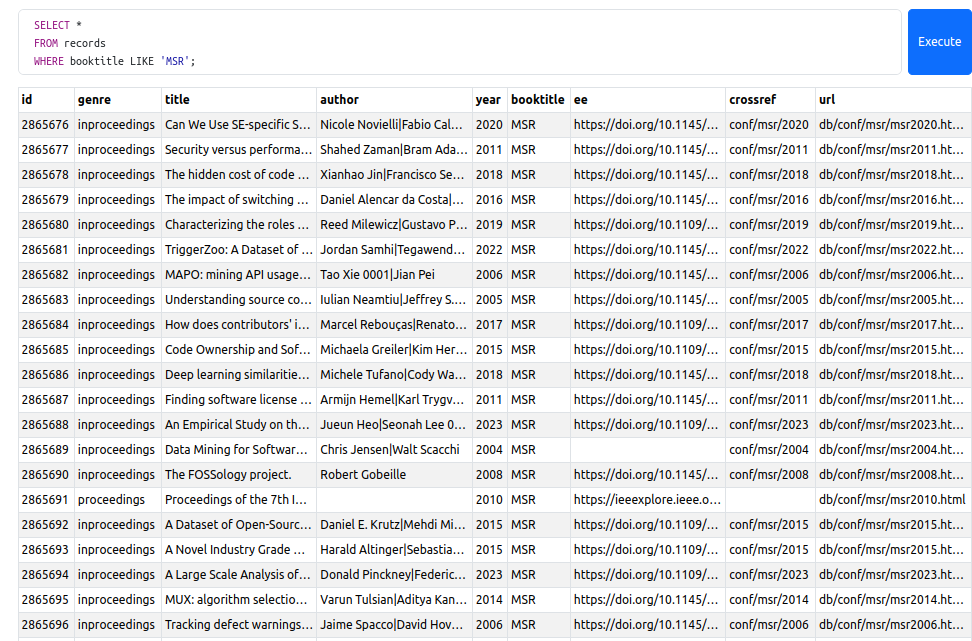
\includegraphics[width=11.5cm, keepaspectratio]{img/ej_sqlite_MSR.png}
  \caption{Ejemplo de resultados base datos MSR}
  \label{fig:ej_sqlite}
\end{figure}

En la siguiente figura se puede observar un ejemplo del congreso MSR concretando el autor 'Gregorio Robles':

\begin{figure}[h]
  \centering
  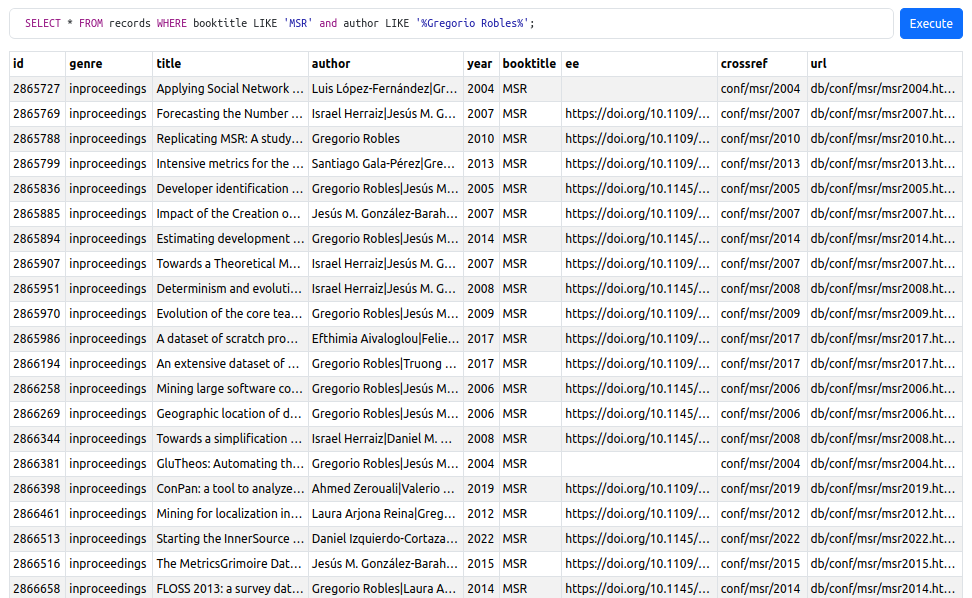
\includegraphics[width=11.5cm, keepaspectratio]{img/ej_bd_GR.png}
  \caption{Ejemplo de resultados base de datos Gregorio Robles}
  \label{fig:ej_GR}
\end{figure}

Como es tedioso y nada intuitivo no se pueden presentar datos de manera efectiva de visualización en un solo vistazo es por ello que se busca el siguiente paso, que es la de extraer los datos concretos de congresos, en un principio por congreso-archivo y en un siguiente paso varios congresos por archivo.

En este punto se desarrolló un código para realizar el conteo de las apariciones de los autores y mas tarde su comparación por congresos, mas detallado en el punto 4.2.5.
Se realizó antes de conocer que habría que implementar un visor de los datos como el que se llevo a cabo en este trabajo. Para exponer los resultados se ha tomado de ejemplo los congreos MSR y ICSME:

\begin{figure}[h]
    \centering
    \begin{tabular}{cc}
    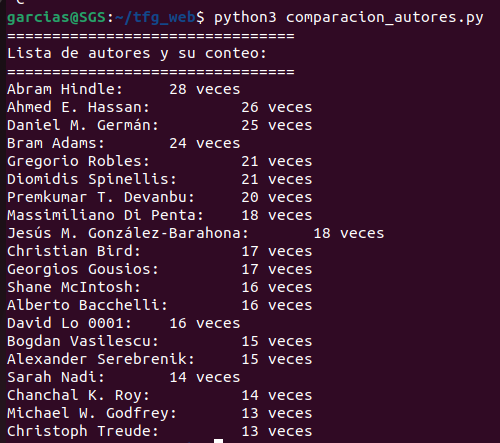
\includegraphics[width=0.595\textwidth]{img/MSR_list_count.png} &  
    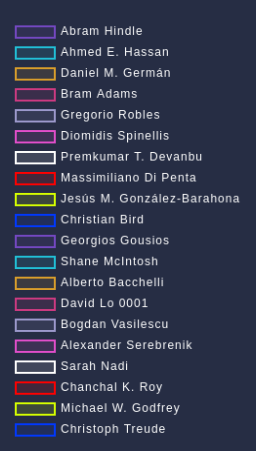
\includegraphics[width=0.3\textwidth]{img/MSR_list_l.png} \\
    (a) &(b)
    \end{tabular}
    \caption{(a) Listado comparación de autores por terminal (b) Resultado Web.}
    \label{fig:comp_MSR}
\end{figure}


Como se puede observar la herramienta de comparación de autores, concretando en el listado de los 20 autores que más aparecen, se puede observa una similitud en los datos, esto refleja que ambos códigos extraen los datos de manera efectiva y se encuentra similitud entre ambos. 

En la imagen (b) de la figura ~\ref{fig:comp_MSR} se aprecia la jerarquia de las apariciones, se puede comparar con el la imágen (a) de la misma figura, pero no se observan el número de apariciones, este dato se obtiene de manera interactiva en el gráfico, pudiendo colocar el ratón por encima del dato en el gráfico apareciendo el valor como se puede apreciar en la figura ~\ref{fig:msr_inter}, del mismo modo en dicha figura se puede apreciar un valor estimado según las alturas de los datos.

\begin{figure}[!h]
  \centering
  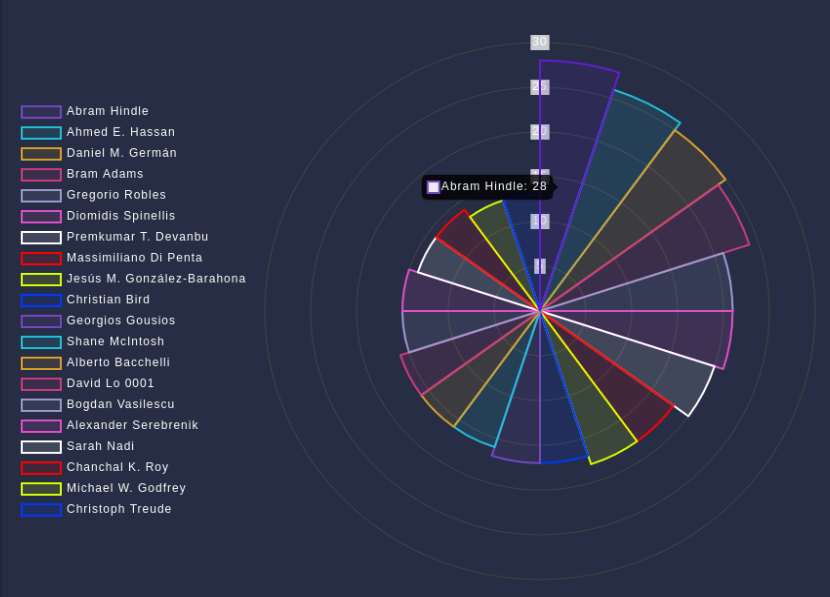
\includegraphics[width=14cm, keepaspectratio]{img/MSR_interactive.png}
  \caption{Gráfico apariciones MSR}
  \label{fig:msr_inter}
\end{figure}

\begin{figure}[!h]
    \centering
    \begin{tabular}{cc}
    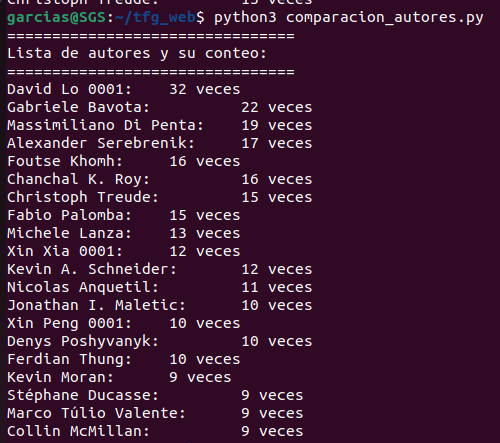
\includegraphics[width=0.595\textwidth]{img/ICSME_list_count.png} &  
    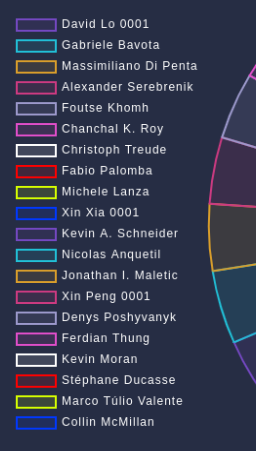
\includegraphics[width=0.3\textwidth]{img/ICSME_list_l.png} \\
    (a) &(b)
    \end{tabular}
    \caption{(a) Listado comparación de autores por terminal (b) Resultado Web.}
    \label{fig:comp_ICSME}
\end{figure}

Lo mismo ocurre con los datos del congreso ICSME, como se puede ver en la figura ~\ref{fig:comp_ICSME}

Una vez se ha obtenido el ranking de los 20 autores que mas aparecen por congreso tenemos como misión la comparación de las apariciones de los autores respecto a los dos congresos, se lleva a cabo mediante la intersección de los datos de ambos congresos:

\begin{figure}[!h]
    \centering
    \begin{tabular}{cc}
    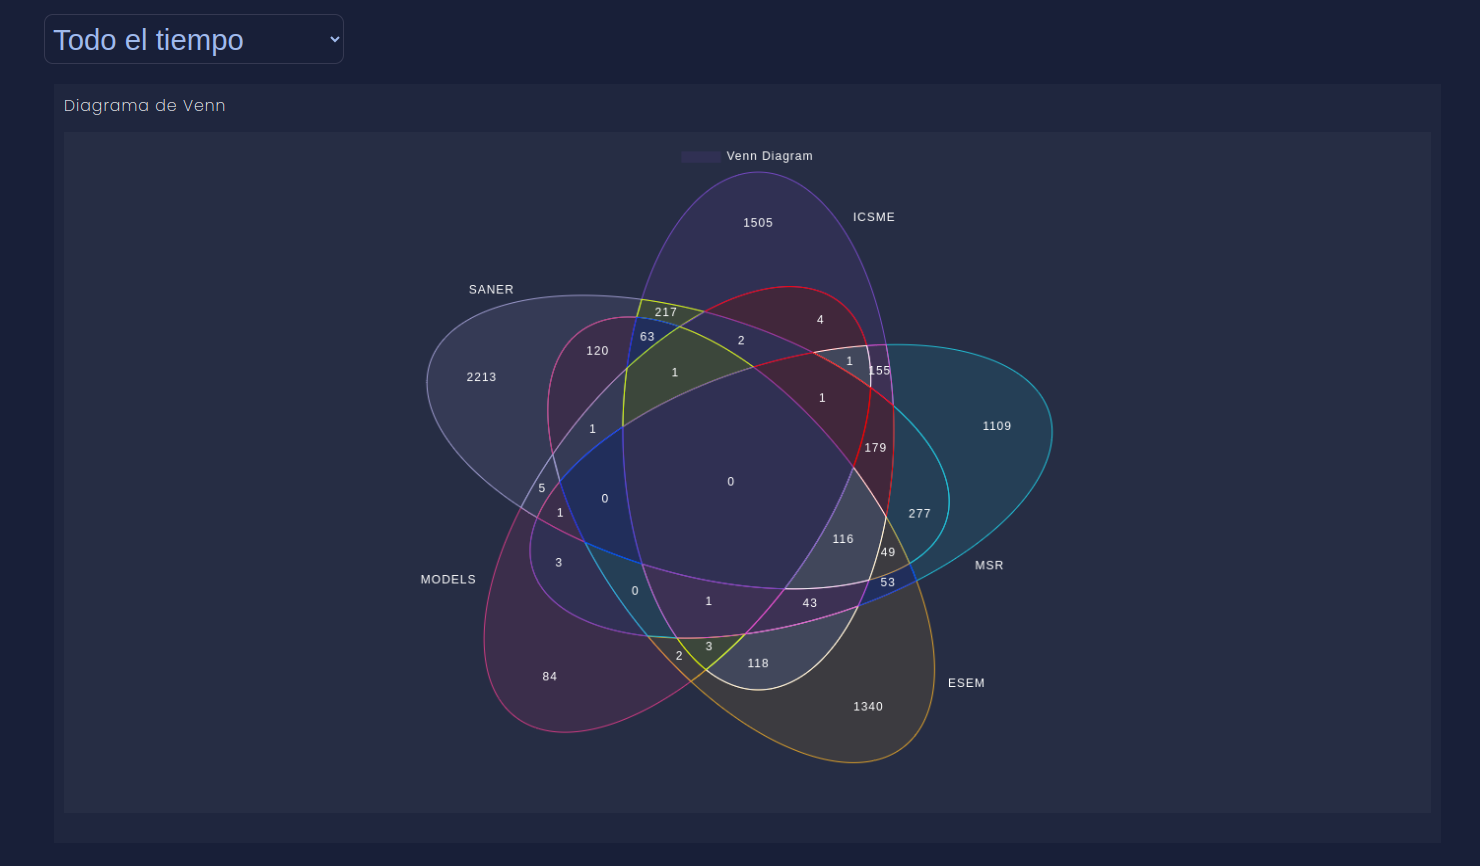
\includegraphics[width=0.595\textwidth]{img/venn_graph_T.png} &  
    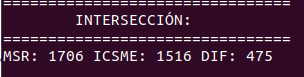
\includegraphics[width=0.3\textwidth]{img/inter_all.png} \\
    (a) &(b)
    \end{tabular}
    \caption{Intersección entre congresos (a) gráficamente y (b) herramienta de análisis.}
    \label{fig:comp_inter_all}
\end{figure}

En la figura ~\ref{fig:comp_inter_all}, se observa una diferencia en la intersección, debido a que a la hora de mostrar los datos por terminal, evitamos los autores que aparecen como vacíos.

De manera adicional, se exponen las diferencias que se encuentran entre la aplicación del trabajo y la herramienta de pruebas para los valores del desplegable web. Igual que ocurre con la presentación total de los datos, cada gráfico se verá actualizado con los valores nuevos tal y como se desarrolló en el apartado 4.2.4.

\subsubsection{Un año:}
Tras seleccionar del desplegable la opción "1 año", se actualizan los gráficos con los autores que aparecen por congreso y la intersección del último año, según se puede ver en la figura ~\ref{fig:comp_msr_1_year} del apéndice, se observa la similitud en los datos obtenidos en ambas partes. En el gráfico de ICSME, se caracteriza por obtener una aparición parecida entre autores, muy diferente con el gráfico de MSR, el cual se observa como destacan varios autores con más apariciones.

Destacable es la baja aparición en la intersección de ambos congresos con solo 22 similitudes entre ambos.


\subsubsection{Cinco años:}
Como ocurre en el caso anterior, tras seleccionar la opción "5 años" se obtiene los datos correspondientes a ambos congresos. En este punto se puede observar que la aparición de autores por congresos ha aumentado considerablemente respecto los valores anteriores en ambos congresos.

A destacar que han aumentado de un 10\% de similitudes en el caso anterior a casi mas del 25\% en esta selección en cuanto a la intersección entre ambos congresos.


\subsubsection{Diez años:}
Para esta selección de datos, se puede observar la tendencia al alza de apariciones de autores por congresos, que comparándolo con las apariciones totales de los autores por congresos no cambian considerablemente los valores entre ellos. Esta afirmación se puede observar en las figuras ~\ref{fig:comp_icsme_10_year}, ~\ref{fig:comp_msr_10_year} y ~\ref{fig:res_web}

La intersección de autores entre los congresos en este selector aumenta hasta casi el 35\% respecto los dos congresos.

\begin{figure}[h]
  \centering
  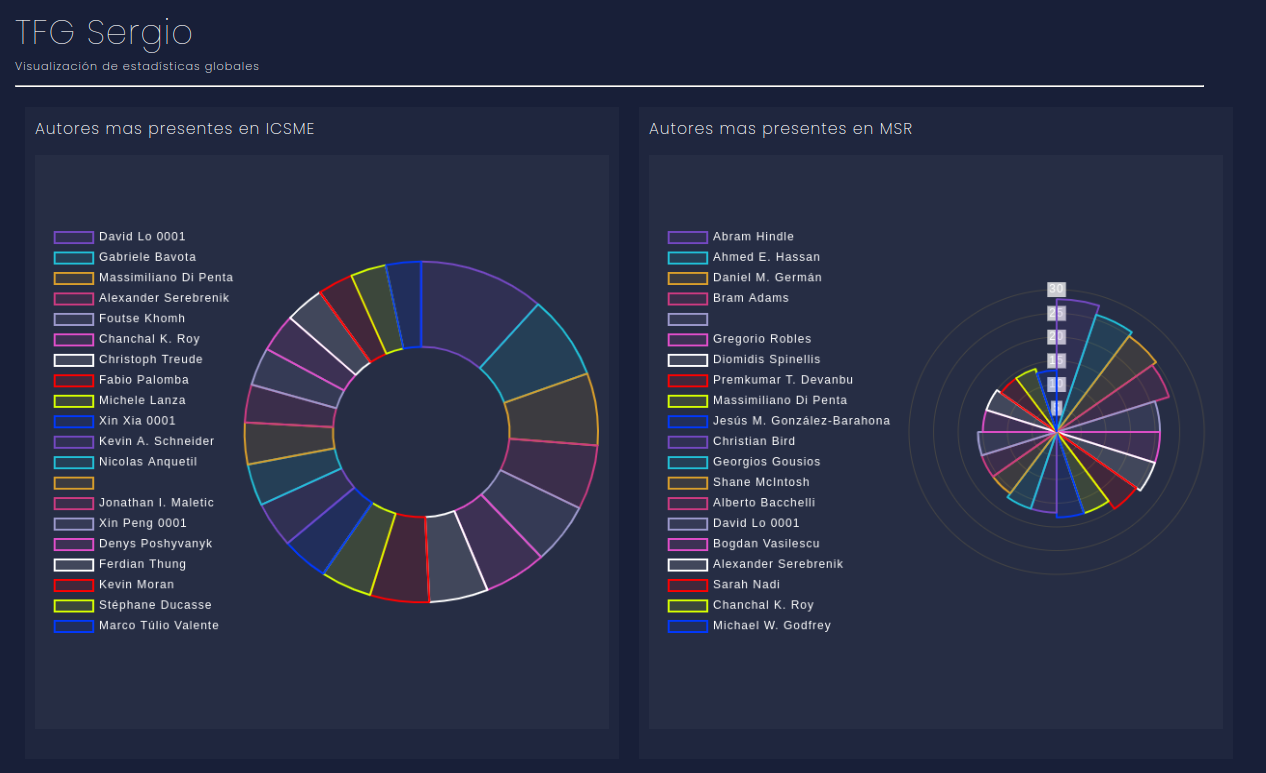
\includegraphics[width=16cm, keepaspectratio]{img/res_web.png}
  \caption{Ejemplo de resultados en web}
  \label{fig:res_web}
\end{figure}


%%%%%%%%%%%%%%%%%%%%%%%%%%%%%%%%%%%%%%%%%%%%%%%%%%%%%%%%%%%%%%%%%%%%%%%%%%%%%%%%
%%%%%%%%%%%%%%%%%%%%%%%%%%%%%%%%%%%%%%%%%%%%%%%%%%%%%%%%%%%%%%%%%%%%%%%%%%%%%%%%
% CONCLUSIONES %
%%%%%%%%%%%%%%%%%%%%%%%%%%%%%%%%%%%%%%%%%%%%%%%%%%%%%%%%%%%%%%%%%%%%%%%%%%%%%%%%

\cleardoublepage
\chapter{Conclusiones}
\label{chap:conclusiones}
\section{Consecución de objetivos}
\label{sec:consecucion-objetivos}

En esta sección vamos a contrastar lo expuesto en la sección de objetivos del proyecto, aunque a grandes rasgos se puede decir que se han conseguido los objetivos que allí se proponían.

Como punto de partida, había que decidir la metodología, las tecnologías que se utilizarían y el proceso a llevar. Se ha conseguido definir un flujo de trabajo cómodo y por partes que facilitaría el manejo de datos y su posterior visualización. Ha sido un acierto utilizar el lenguaje Python para las tareas de parseo del XML, para el manejo y extracción de datos concretos de la base de datos y su posterior volcado en JSON. Nos aportó una versatilidad que probablemente otras herramientas nos hubiera resultado mas complejas.

Por otra parte, otro de los objetivos cumplidos es el desarrollo de la herramienta de visualización de datos. Destacar en este punto que ha sido parte de la implementación mas compleja del proyecto, ya que el manejo de los datos recibidos de una API no se trata dentro del grado y he tenido que tener un aprendizaje para la consecución del objetivo. 

Para finalizar con los objetivos del apartado 2, tenemos el ámbito de las pruebas y comparaciones de resultados. Apartado importante para contrastar la información que se obtenía gráficamente con la obtenida de la herramienta de test. Muy nutritivo este objetivo, ya que me ha aportado conocimiento para implementar una herramienta que se ajustara a los parámetros del proyecto y así realizar una comprobación correcta.
También hacer incapié en la necesidad de esta herramienta para conocer los fallos y las necesidades que me requería el apartado visual.

Queda hacer referencia a una frase de la web dblp.org\footnote{\url{https://dblp.org/faq/1474635.html}}: \textit{Not everything that can be counted counts, and not everything that counts can be counted."} En la que nos hace tener en cuenta que en este proyecto se ha sintetizado los datos para exponer concretamente los más necesarios.



% \begin{verbatim}
%   aspell --lang=es_ES -c memoria.tex
% \end{verbatim}

\section{Aplicación de lo aprendido}
\label{sec:aplicacion}

En este apartado se va a detallar los aprendizajes obtenidos en el grado y como se ha aplicado a este Trabajo de Fin de Grado.

\begin{enumerate}
  \item Informática I: En esta asignatura aprendí los fundamentos de programación, me aportó una base y un primer contacto en el mundo de la programación.
  \item Arquitectura de Internet: En esta asignatura, me aportó las bases de las redes y los protocolo de red, para este trabajo nos ayuda a conocer como se realiza la transferencia de los datos para visualizarlos.
  \item Informática II: En esta asignatura se centró mas en aportarnos la base sobre algorítmos y como se realizaban las buenas prácticas de programación.
  \item Sistemas Telemáticos para Medios Audiovisuales: En esta asignatura se profundiza sobre comunicación de red y protocolos, en este trabajo se aplica sobre la comunicación HTTP que se realiza para obtener los datos de la API.
  \item Protocolos para la Transmisión de Audio y Video en Internet: Es la asignatura donde comenzamos a utilizar Python, aprendemos la programación orientada a objetos, nociones de estilo de código y algorítmos, en este trabajo se utiliza para el comienzo del trabajo, en el cual se extráen los datos para obtener una base de datos, posteriormente se utiliza para sintetizar esa base de datos en un JSON con los datos solicitados y para realizar el código de test.
  \item Arquitectura de sistemas II: En esta asignatura aprendí sobre la programación a bajo nivel, me hizo entender como funciona la programación y la importancia de los lenguajes de alto nivel como Python.
  \item Construcción de servicios y aplicaciones audiovisuales en internet: Asignatura que nos daba las nociones de HTML, HTML5, CSS, JavaScrip... Muy utilizado en este trabajo para la parte visual de los datos.
  \item Laboratorio de Tecnologías Audiovisuales en la web: Asignatura en la que profundizamos en tecnologías aplicadas en la web.
  \item Graficos y visualización 3D: Igual que ocurre con las anteriores asignaturas, aprendí el funcionamiento de la etiqueta <canva> y como se puede visualizar datos.
\end{enumerate}

Por último, queda hacer mención sobre el resto de asignaturas que de una forma u otra me han ayudado en este trabajo, asignaturas arduas que me enseñaron que es el esfuerzo, como asignaturas que enseñaban la organización. Destacar del mismo modo las asignaturas que me hicieron presentar, eso me ayudará en la presentación de este trabajo, haciendo mención especial a la asignatura expresión oral y escrita y busqueda de información, en la cual nos enseñaron las herramientas de búsqueda, así como la forma de exponer. Gracias a todas estas y demás asignaturas me han ayudado a estar en este momento.

\section{Lecciones aprendidas}
\label{sec:lecciones_aprendidas}

En este apartado toca reflexionar sobre los aprendizajes que me ha aportado el trabajo, destacar que ha sido un recorrido en el cual he aprendido en todo momento.

\begin{enumerate}
  \item El concepto de organización: Me ha aportado la capacidad de organizar un proyecto, conocer las fases para llevarlo a cabo y seguirlo de manera correcta. Saber poner subtareas e ir creando este trabajo pieza por pieza.
  \item Mayor conocimiento de las herramientas utilizadas: Gracias a este trabajo he podido mantener el contacto con el mundo de la programación, he trabajado con varias tecnologías y eso me ha ayudado a obtener mas conocimiento.
  \item Conocimiento de tecnologías nuevas: Se han desarrollado códigos y se ha implementado una solución en la cual he tenido que aprender según he ido encontrando dificultades. 
  Se ha aprendido el funcionamiento de la funcionalidad API y como obtener datos de ella, por ejemplo.
  \item Capacidad de contrastar el proyecto principal con test: Gracias a este trabajo he podido ampliar mi conocimiento sobre realizar test, al mismo modo he confirmado mi capacidad para realizarlos.
  \item Afianzar conocimientos sobre GitHub: Una vez que he llevado a cabo el proyecto he podido comprobar lo útil y necesario que es utilizar esta plataforma. He podido comenzar un repositorio y llevarlo a buen puerto.
  \item Conocimiento de \LaTeX, el cual me ha dado quebraderos de cabeza en un comienzo, pero muy potente como herramienta, ya que prácticamente te hace el trabajo de maquetado solo.
\end{enumerate}


\section{Trabajos futuros}
\label{sec:trabajos_futuros}

Este proyecto puede ser mejorado en varios aspectos que se detallan de la siguiente manera:

\begin{enumerate}
    \item Para comenzar, la primera mejora que se propone es la de alojar el entorno web en un servidor online, de esta manera poderla consultar desde cualquier lado y sin limitaciones de instalaciones de librerías y dependencias.
    \item Realizar la herramienta de parseo XML online (como ocurre con https://inloop.github.io/sqlite-viewer/), tener la herramienta online liberaría de carga de cómputo y memoria a la máquina en la que se parsea el documento. Pudiéndose pasar como parámetro la URL del documento a parsear o un archivo. Una vez obtenido esto ofrecer la opción de extraer los datos concretos a JSON.
    \item Ampliación de la herramienta de visualización de datos y proponer al usuario mas opciones con las que visualizar datos, como por ejemplo: permitir al usuario elegir que tipo de gráfico quiere utilizar o implementar una funcionalidad por intervalo de años.
    
\end{enumerate}


%%%%%%%%%%%%%%%%%%%%%%%%%%%%%%%%%%%%%%%%%%%%%%%%%%%%%%%%%%%%%%%%%%%%%%%%%%%%%%%%
%%%%%%%%%%%%%%%%%%%%%%%%%%%%%%%%%%%%%%%%%%%%%%%%%%%%%%%%%%%%%%%%%%%%%%%%%%%%%%%%
% APÉNDICE(S) %
%%%%%%%%%%%%%%%%%%%%%%%%%%%%%%%%%%%%%%%%%%%%%%%%%%%%%%%%%%%%%%%%%%%%%%%%%%%%%%%%

\cleardoublepage
\appendix
\chapter{Gráficos de resultados.}
\label{app:manual}

Este apartado es para mostrar las evidencias gráficas del apartado de resultados:

\begin{figure}[!h]
    \centering
    \begin{tabular}{cc}
    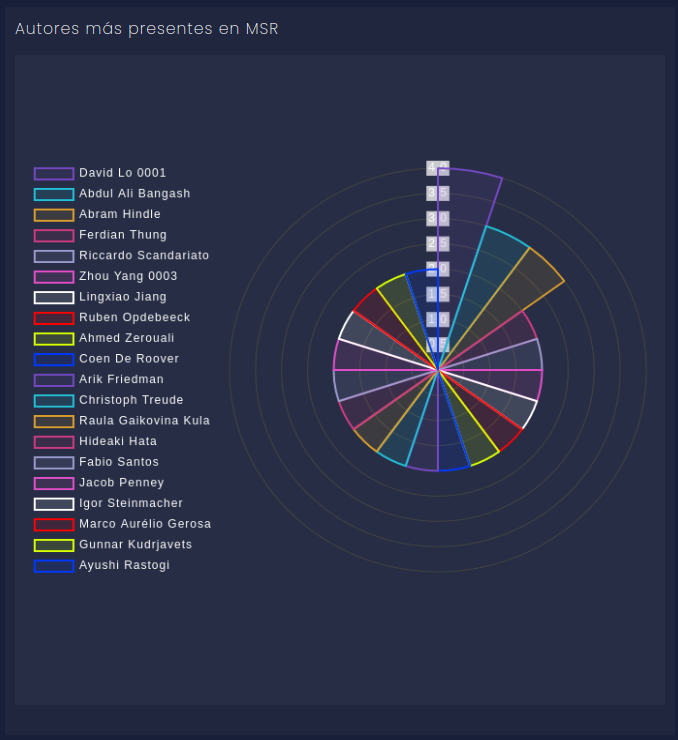
\includegraphics[width=0.45\textwidth]{img/msr_1_year_graph.png} &  
    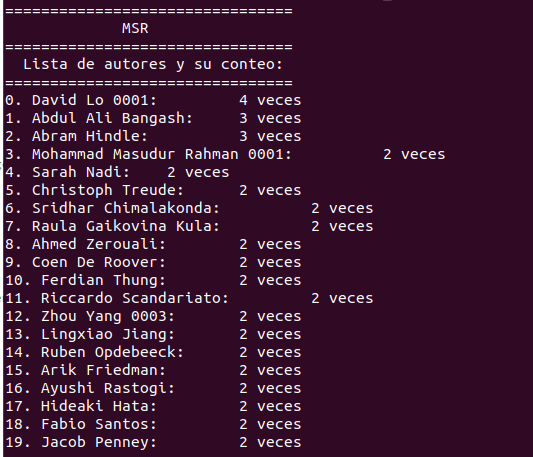
\includegraphics[width=0.52\textwidth]{img/msr_1_year.png} \\ 
    (a) &(b) 
    \end{tabular}
    \caption{Valores MSR de 1 año (a) gráficamente y (b) herramienta de análisis.}
    \label{fig:comp_msr_1_year}
\end{figure}

\begin{figure}[!h]
    \centering
    \begin{tabular}{cc}
    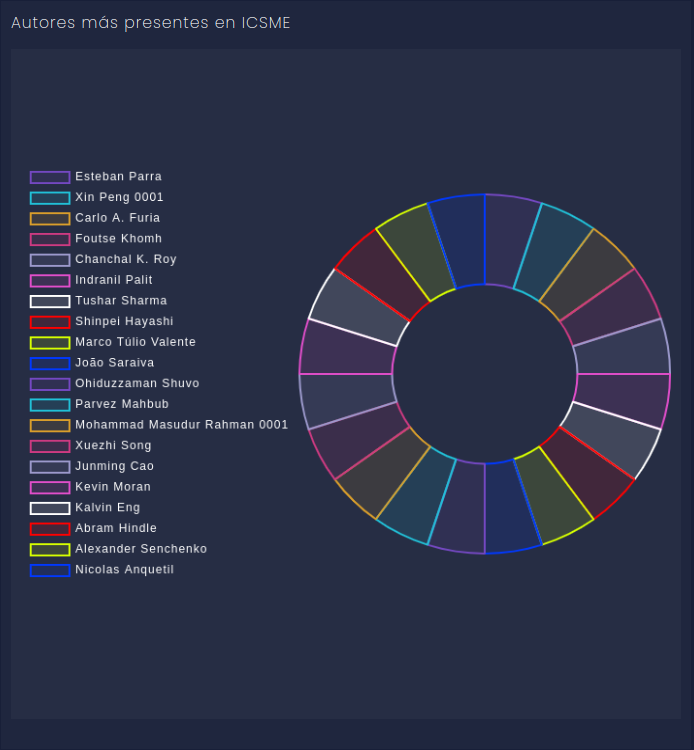
\includegraphics[width=0.45\textwidth]{img/icsme_1_year_graph.png} &  
    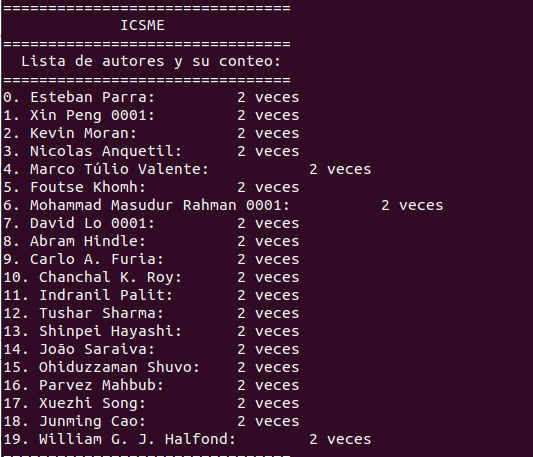
\includegraphics[width=0.52\textwidth]{img/icsme_1_year.png} \\ 
    (a) &(b) 
    \end{tabular}
    \caption{Valores ICSME de 1 año (a) gráficamente y (b) herramienta de análisis.}
    \label{fig:comp_icsme_1_year}
\end{figure}

\begin{figure}[h]
  \centering
  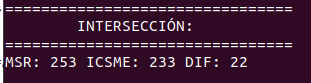
\includegraphics[width=8cm, keepaspectratio]{img/inter_1_year.png}
  \caption{Intersección ICSME-MSR 1 año.}
  \label{fig:inter_1_year}
\end{figure}

\begin{figure}[!h]
    \centering
    \begin{tabular}{cc}
    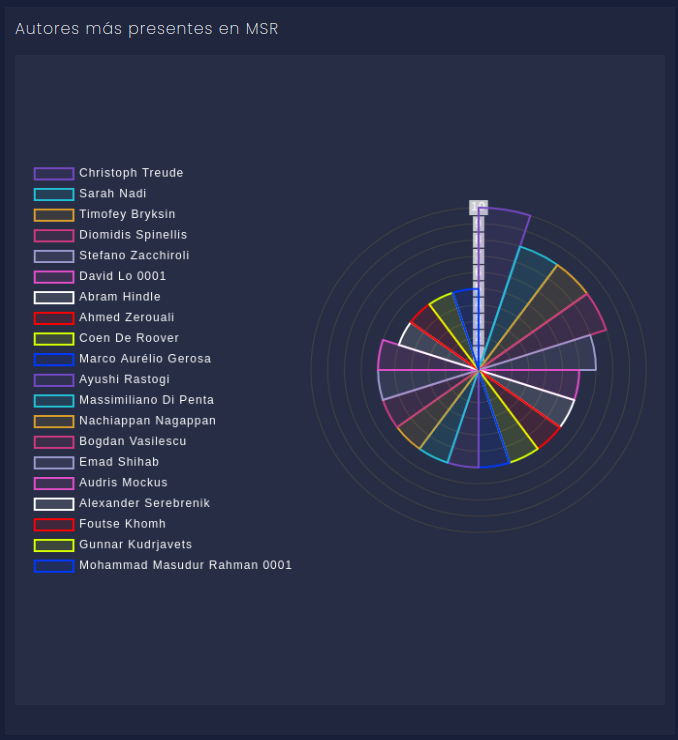
\includegraphics[width=0.45\textwidth]{img/msr_5_year_graph.png} &  
    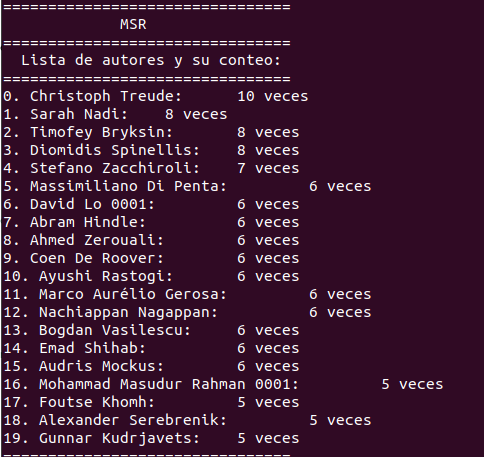
\includegraphics[width=0.52\textwidth]{img/msr_5_year.png} \\ 
    (a) &(b) 
    \end{tabular}
    \caption{Valores MSR de 5 años (a) gráficamente y (b) herramienta de análisis.}
    \label{fig:comp_msr_5_year}
\end{figure}

\begin{figure}[!h]
    \centering
    \begin{tabular}{cc}
    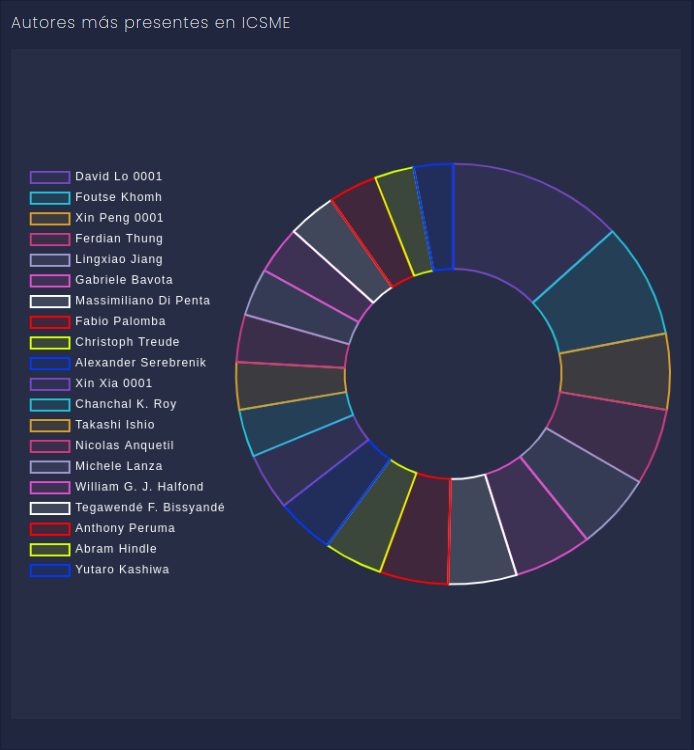
\includegraphics[width=0.45\textwidth]{img/icsme_5_year_graph.png} &  
    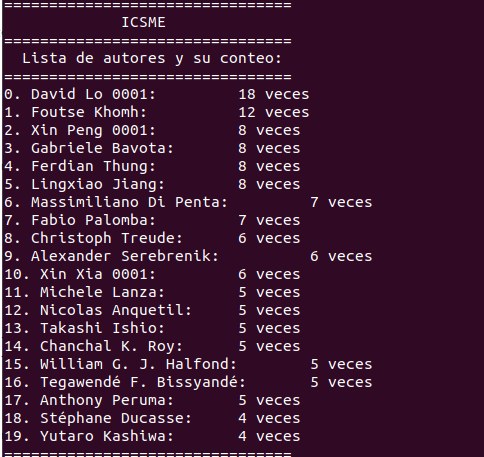
\includegraphics[width=0.52\textwidth]{img/icsme_5_year.png} \\ 
    (a) &(b) 
    \end{tabular}
    \caption{Valores ICSME de 5 años (a) gráficamente y (b) herramienta de análisis.}
    \label{fig:comp_icsme_1_year}
\end{figure}

\begin{figure}[h]
  \centering
  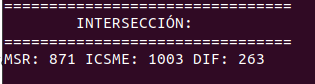
\includegraphics[width=8cm, keepaspectratio]{img/inter_5_year.png}
  \caption{Intersección ICSME-MSR 5 año.}
  \label{fig:inter_5_year}
\end{figure}

\begin{figure}[!h]
    \centering
    \begin{tabular}{cc}
    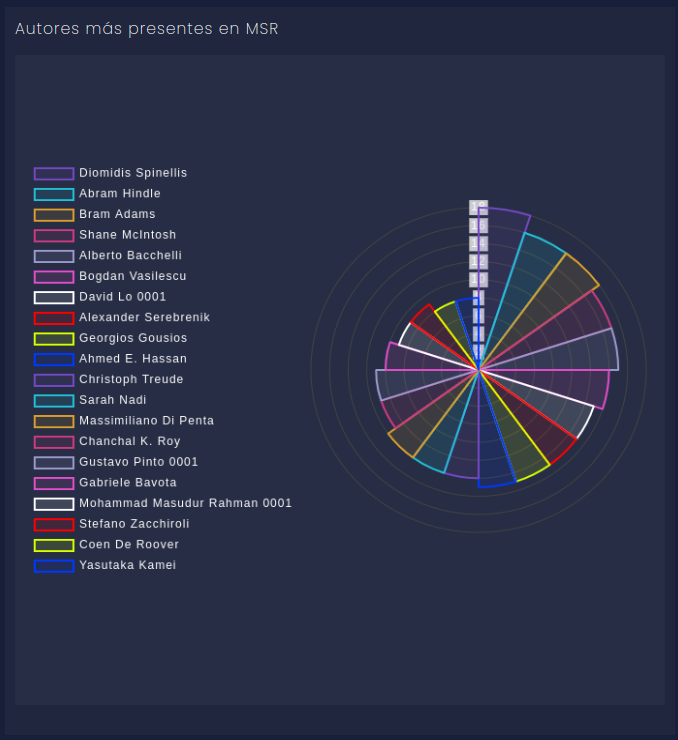
\includegraphics[width=0.45\textwidth]{img/msr_10_year_graph.png} &  
    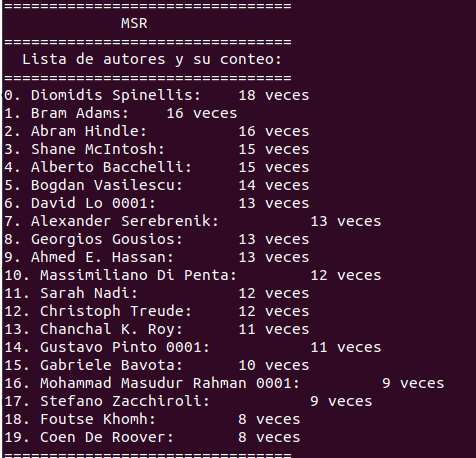
\includegraphics[width=0.52\textwidth]{img/msr_10_year.png} \\ 
    (a) &(b) 
    \end{tabular}
    \caption{Valores MSR de 10 años (a) gráficamente y (b) herramienta de análisis.}
    \label{fig:comp_msr_10_year}
\end{figure}

\begin{figure}[!h]
    \centering
    \begin{tabular}{cc}
    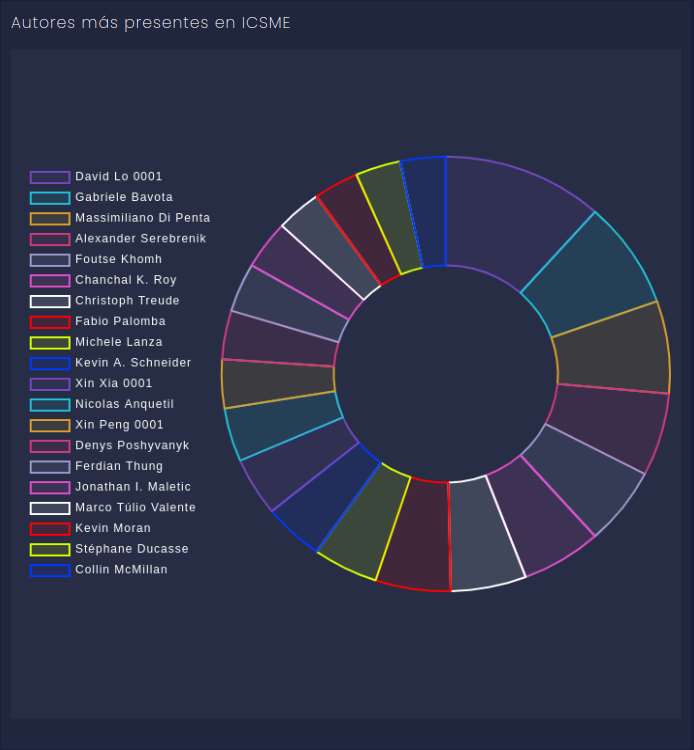
\includegraphics[width=0.45\textwidth]{img/icsme_10_year_graph.png} &  
    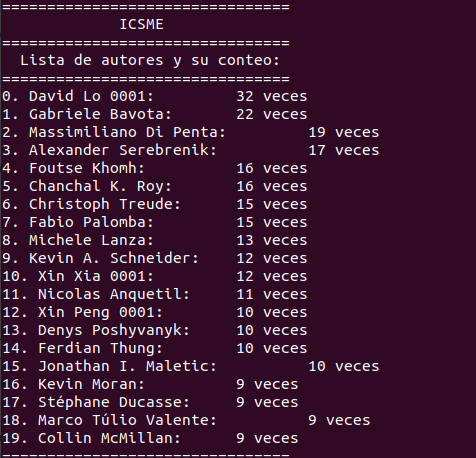
\includegraphics[width=0.52\textwidth]{img/icsme_10_year.png} \\ 
    (a) &(b) 
    \end{tabular}
    \caption{Valores ICSME de 10 años (a) gráficamente y (b) herramienta de análisis.}
    \label{fig:comp_icsme_10_year}
\end{figure}

\begin{figure}[h]
  \centering
  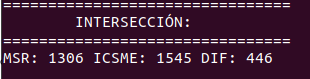
\includegraphics[width=8cm, keepaspectratio]{img/inter_10_year.png}
  \caption{Intersección ICSME-MSR 10 año.}
  \label{fig:inter_10_year}
\end{figure}


%%%%%%%%%%%%%%%%%%%%%%%%%%%%%%%%%%%%%%%%%%%%%%%%%%%%%%%%%%%%%%%%%%%%%%%%%%%%%%%%
%%%%%%%%%%%%%%%%%%%%%%%%%%%%%%%%%%%%%%%%%%%%%%%%%%%%%%%%%%%%%%%%%%%%%%%%%%%%%%%%
% BIBLIOGRAFIA %
%%%%%%%%%%%%%%%%%%%%%%%%%%%%%%%%%%%%%%%%%%%%%%%%%%%%%%%%%%%%%%%%%%%%%%%%%%%%%%%%

\cleardoublepage

% Las siguientes dos instrucciones es todo lo que necesitas
% para incluir las citas en la memoria
\bibliographystyle{abbrv}
\bibliography{memoria}  % memoria.bib es el nombre del fichero que contiene
% las referencias bibliográficas. Abre ese fichero y mira el formato que tiene,
% que se conoce como BibTeX. Hay muchos sitios que exportan referencias en
% formato BibTeX. Prueba a buscar en http://scholar.google.com por referencias
% y verás que lo puedes hacer de manera sencilla.
% Más información: 
% http://texblog.org/2014/04/22/using-google-scholar-to-download-bibtex-citations/

\end{document}
